\documentclass[letterpaper, 12pt]{article}
% \usepackage[showframe, margin=1in, top=0.25in, bottom=0.25in, includeheadfoot, headheight=0.5in]{geometry}
\usepackage[margin=1in, top=0.25in, bottom=0.25in, includeheadfoot, headheight=0.5in]{geometry}

\AddToHook{cmd/section/before}{\clearpage}

\usepackage[table]{xcolor}
\colorlet{listingback}{gray!20}
\definecolor{headingcolor}{RGB}{110,34,54}

\usepackage{fancyhdr}
\renewcommand{\sectionmark}[1]{\markboth{#1}{#1}}

% Used to detect whether a section is an appendix to print the right thing in the footer
\usepackage{etoolbox}
\newtoggle{inappendix}
\pretocmd{\appendix}{\clearpage\toggletrue{inappendix}}{}{}

% Save standard definitions for head and foot rules (lines separating header and footer from text)
\let\HeadRule\headrule
\let\FootRule\footrule
% Add color to the standard definitions
\renewcommand{\headrule}{\color{headingcolor}\HeadRule}
\renewcommand{\footrule}{\textcolor{headingcolor}{\FootRule}}

% IMPORTANT: This command should not be called directly. Use \preamble.
% Macro to insert the title page for each lab.
% The argument is the title of the lab.
\newcommand{\inserttitlepage}[1]
{
    \begin{titlepage}
    \centering
    
\includegraphics[scale=0.5]{images/nexus_lab_logo.png}

    \vspace*{\baselineskip}

    \textbf{\Large OpenStack Labs}

    \vspace*{\baselineskip}

    \textbf{\Large #1}
    \vspace*{\fill}
\end{titlepage}
}

% IMPORTANT: This command should not be called directly. Use \preamble.
% Macro to define header and footer for each lab.
% The argument is the title of the lab.
\newcommand{\headfoot}[1]
{
    \fancypagestyle{fancy}
    {
        \fancyhf{}
        \fancyhead[L]{\footnotesize #1}
        \fancyhead[R]{
\includegraphics[height=0.85\headheight]{images/nexus_lab_logo.png}}
        \fancyfoot[L]{%
            \footnotesize%
            \ifnum\value{section}>0%
            \iftoggle{inappendix}{Appendix \thesection: \rightmark}{Section \thesection: \rightmark}%
            \fi}
        \fancyfoot[R]{\footnotesize\thepage}
        \renewcommand{\headrulewidth}{1.5pt}
        \renewcommand{\footrulewidth}{1.5pt}
    }
}

% Macro to insert title page, define header and footer, and insert table of contents and about section for each lab.
% The argument is the title of the lab.
\newcommand{\preamble}[1]
{
    \pagenumbering{roman}
    \inserttitlepage{#1}
    \headfoot{#1}

    % Insert table of contents
    \pagestyle{fancy}
    \tableofcontents
    \clearpage

    \section*{About This Document}
    \label{sec:about_this_document}
    \begin{itemize}
        \item This document was developed by a team at the University of Tennessee at Chattanooga led by Dr. Mengjun Xie
        (\href{mailto:mengjun-xie@utc.edu}{\textbf{mengjun-xie@utc.edu}}).
        \item The development of this document was supported by a National Centers of Academic Excellence in Cybersecurity Grant (\#H98230-20-1-0351), housed at the National Security Agency.
        \item This document is licensed with a Creative Commons Attribution 4.0 International License.
    \end{itemize}
    \clearpage
}

% Macro to insert the Lab Settings page for each lab. Call after the Introduction and Objectives sections.
\newcommand{\labsettings}
{
    \section*{Lab Settings}
    \label{sec:lab_settings}
    \addcontentsline{toc}{section}{\nameref{sec:lab_settings}}
    The information in the table below will be needed in order to complete the lab.
    The task sections below provide details on the use of this information.
    \begin{table*}[htbp]
        \centering
        \begin{tabular}{|c|c|c|c|}
            \hline
            \rowcolor{gray!20} \textbf{Virtual Machine} & \textbf{IP Address} & \textbf{Account} & \textbf{Password} \\
            \hline
            \multirow{2}{*}{\texttt{workstation}} & \multirow[t]{2}{*}{\texttt{ens3: 192.168.1.21}}  & \multirow{2}{*}{\texttt{ubuntu}} & \multirow{2}{*}{\texttt{ubuntu}} \\
                                                  & \multirow[t]{2}{*}{\texttt{ens4: 172.25.250.21}} &                                  &                                  \\
            \hline
            \multirow{2}{*}{\texttt{devstack}}    & \multirow[t]{2}{*}{\texttt{ens3: 192.168.20}}    & \multirow{2}{*}{\texttt{ubuntu}} & \multirow{2}{*}{\texttt{ubuntu}} \\
                                                  & \multirow[t]{2}{*}{\texttt{ens4: 172.25.250.20}} &                                  &                                  \\
            \hline
        \end{tabular}
    \end{table*}
    \clearpage

    % IMPORTANT(lucas): If another frontmatter section ever gets placed after this, this command needs to be moved
    % to the end of that section.
    % I have placed this here and not in each lab purely for convenience and to ensure I don't forget any.
    \pagenumbering{arabic}
}

% Sans-serif font
\renewcommand{\familydefault}{\sfdefault}
\newcommand{\texttildemid}{{\raisebox{0.5ex}{\texttildelow}}}

\usepackage{enumitem}
\renewcommand{\labelenumi}{\textbf{\thesection.\arabic{enumi}.}}

% Try to forbid widows and orphans
\widowpenalty10000
\clubpenalty10000

\usepackage{graphicx}
\usepackage{hyperref}
\hypersetup{colorlinks=true,linkcolor=black,urlcolor={[named] headingcolor}}

\usepackage{sectsty}
\sectionfont{\color{headingcolor}}

% Table of Contents
\usepackage{bookmark}
\usepackage[titles]{tocloft}
\usepackage[title]{appendix}
\renewcommand{\cfttoctitlefont}{\Large\bfseries\color{headingcolor}}
\renewcommand{\cftsecfont}{\normalfont\normalsize}
\renewcommand{\cftsecpagefont}{\normalfont\normalsize}
\renewcommand{\cftdotsep}{0} % Make dots small and close together
\renewcommand{\cftsecleader}{\cftdotfill{\cftdotsep}} % Add dots after section titles
% Make dots go all the way to the page number
\renewcommand{\cftsecfillnum}[1]{{\cftsecleader}\nobreak{\cftsecpagefont #1}\cftsecafterpnum\par}

\usepackage{multirow}
\setlength{\tabcolsep}{16pt}
\renewcommand{\arraystretch}{1.1}

% For nice-looking boxes
\usepackage[most]{tcolorbox}
\usepackage{listings}
\usepackage{lstautogobble}
\lstset{
  frame=none,
  language=Bash,
  showstringspaces=false,
  basicstyle={\linespread{1.1}\footnotesize\ttfamily\selectfont},
  numbers=none,
  breaklines=true,
  breakatwhitespace=true,
  tabsize=3,
  columns=fullflexible,
  keepspaces=true,
  escapeinside={(*@}{@*)},
  literate={~}{{\texttildemid}}{1}
           {\#}{\#}{1},
  autogobble=true
}

\tcolorboxenvironment{lstlisting}
{
    spartan,
    colframe=gray!50,
    boxsep=0mm,
    left=1mm,
    right=1mm,
    top=-1mm,
    bottom=-1mm,
    colback=gray!20
}

% Hacky solution for now, would like to have just one environment and make several tcolorboxes by passing different
% colors as parameters, but that is giving errors
\makeatletter
\tcbset{
  note/.style={%
        enhanced,
        breakable,
        colback=blue!10!white,
        colframe=blue!80!white,
        attach boxed title to top left={yshift*=-\tcboxedtitleheight},
        title={#1},
        boxed title size=title,
        boxed title style={%
            sharp corners,
            rounded corners=northwest,
            colback=tcbcolframe,
            boxrule=0pt,
        },
        underlay boxed title={%
            \path[fill=tcbcolframe] (title.south west)--(title.south east)
                to[out=0, in=180] ([xshift=5mm]title.east)--
                (title.center-|frame.east)
                [rounded corners=\kvtcb@arc] |-
                (frame.north) -| cycle;
        },
    }
}
\makeatother

\makeatletter
\tcbset{
    stop/.style={%
        enhanced,
        breakable,
        colback=white,
        colback=red!10!white,
        colframe=red!80!white,
        attach boxed title to top left={yshift*=-\tcboxedtitleheight},
        title={#1},
        boxed title size=title,
        boxed title style={%
            sharp corners,
            rounded corners=northwest,
            colback=tcbcolframe,
            boxrule=0pt,
        },
        underlay boxed title={%
            \path[fill=tcbcolframe] (title.south west)--(title.south east)
                to[out=0, in=180] ([xshift=5mm]title.east)--
                (title.center-|frame.east)
                [rounded corners=\kvtcb@arc] |-
                (frame.north) -| cycle;
        },
    }
}
\makeatother

\makeatletter
\tcbset{
    tip/.style={%
        enhanced,
        breakable,
        colback=white,
        colback=green!10,
        colframe=green!70!black,
        attach boxed title to top left={yshift*=-\tcboxedtitleheight},
        fonttitle=\bfseries,
        title={#1},
        boxed title size=title,
        boxed title style={%
            sharp corners,
            rounded corners=northwest,
            colback=tcbcolframe,
            boxrule=0pt,
        },
        underlay boxed title={%
            \path[fill=tcbcolframe] (title.south west)--(title.south east)
                to[out=0, in=180] ([xshift=5mm]title.east)--
                (title.center-|frame.east)
                [rounded corners=\kvtcb@arc] |-
                (frame.north) -| cycle;
        },
    }
}
\makeatother

% The commands below define environments for colored boxes. They are used like
% \begin{notebox}
% ...
% \end{notebox}
\newtcolorbox{notebox}{note={Note}}
\newtcolorbox{stopbox}{stop={Stop}}
\newtcolorbox{tipbox}{tip={Tip}}

\begin{document}
\preamble{Lab 05: Customizing Instances}

\section*{Introduction}\label{sec:introduction}
\addcontentsline{toc}{section}{\nameref{sec:introduction}}
In this lab, you will use the \textbf{cloud-init} utility to customize OpenStack instances.
This utility is used to perform actions from an instance upon creation.
For example, it can be used to install a list of packages or change the message of the day displayed upon login to the instance.

\section*{Objectives}\label{sec:objectives}
\addcontentsline{toc}{section}{\nameref{sec:objectives}}
\begin{itemize}[itemsep=0pt]
    \item Customize an instance with \textbf{cloud-init} with the \textit{Horizon Dashboard}.
    \item Customize an instance with \textbf{cloud-init} with the \textit{OpenStack Unified CLI}.
    \item Verify instance customization.
\end{itemize}
\clearpage

\labsettings

%%%%%%%%%%%
% Section 1
%%%%%%%%%%%
\section{Setting Up the Environment}\label{sec:setting-up-the-environment}
In this task, you will set up the OpenStack environment to support the customized external instances you will create in the following sections.

\begin{enumerate}
    % TODO: Viewing the default Apache web page will require being able to access the instance from the workstation, which is currently not working
    \begin{labstep}
        Log into the \textbf{workstation} machine as the \textbf{ubuntu} user with password \textbf{ubuntu}.

        \begin{center}
            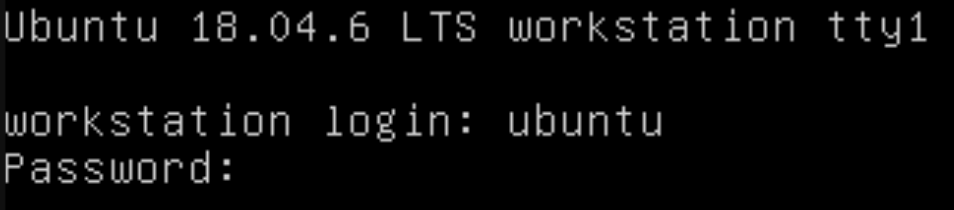
\includegraphics[width=\linewidth]{images/part1/step1.png}
        \end{center}
    \end{labstep}

    \begin{labstep}
        Launch the graphical user interface.
        \begin{lstlisting}
            ubuntu@workstation:~$ startx
        \end{lstlisting}

        \begin{center}
            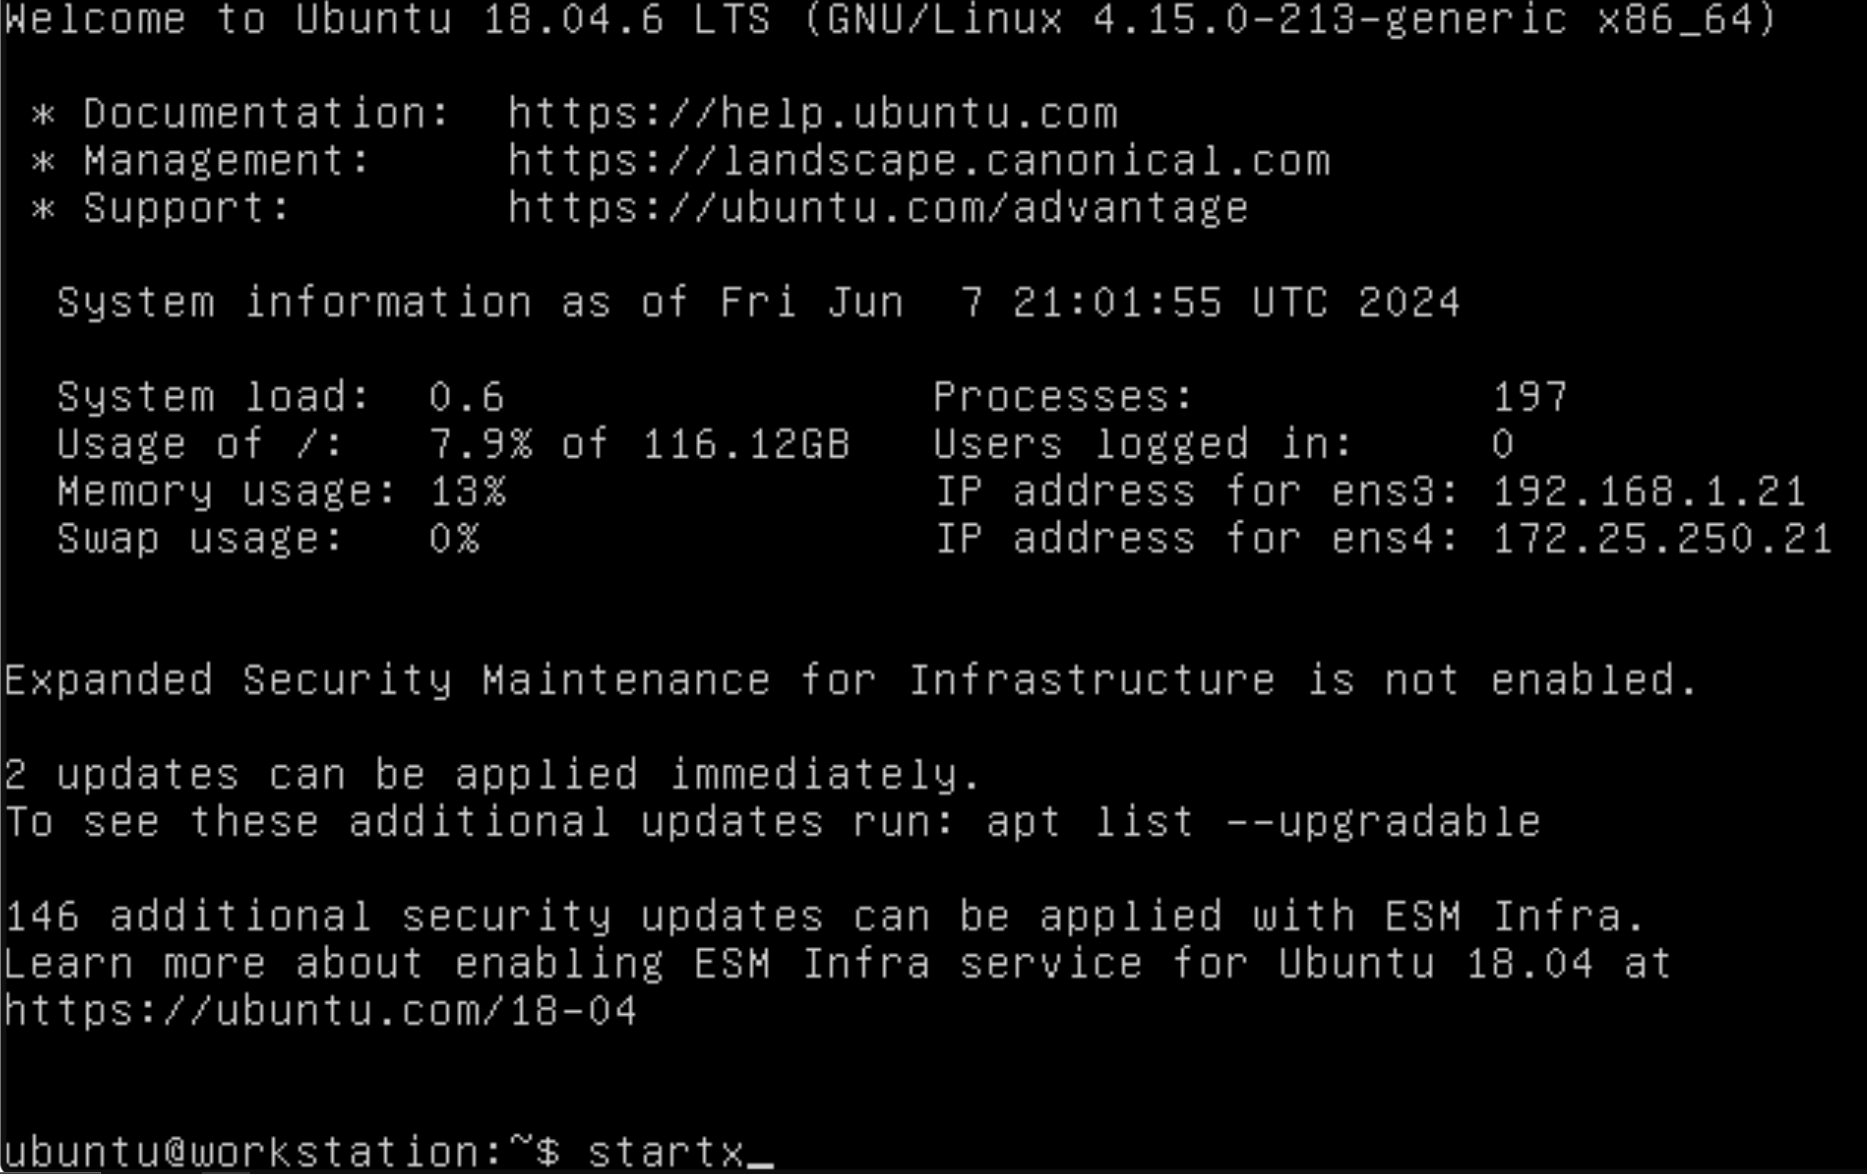
\includegraphics[width=\linewidth]{images/part1/step2.png}
        \end{center}
    \end{labstep}

    \begin{labstep}
        Open a terminal window and source the keystone credentials for the \textbf{admin} user.
        \begin{lstlisting}
            ubuntu@workstation:~$ source ~/keystonerc-admin
        \end{lstlisting}

        \begin{center}
            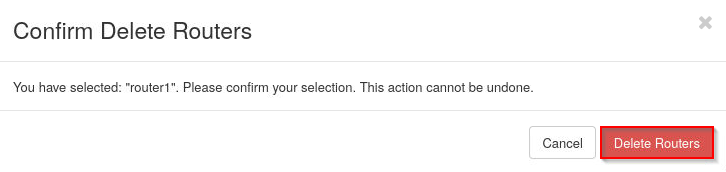
\includegraphics[width=\linewidth]{images/part1/step3.png}
        \end{center}
    \end{labstep}

    \begin{labstep}
        In this lab, we will create our own router and external network.
        First, the default router and external network need to be deleted.
        List the routers to find the default router's name so it can be deleted.
        \begin{lstlisting}
            [ubuntu@workstation (keystone-admin)]:~$ openstack router list
        \end{lstlisting}

        \begin{center}
            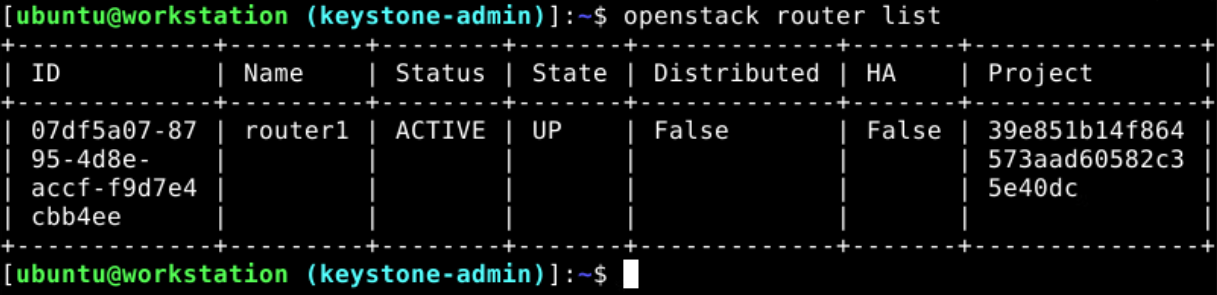
\includegraphics[width=\linewidth]{images/part1/step4.png}
        \end{center}
    \end{labstep}

    \begin{tipbox}
        When typing the command, make sure there is a space between \textbf{list} and the \textbf{\textbackslash} character, and press \textbf{Enter} to get the \textbf{$>$} and continue typing the rest of the command.
    \end{tipbox}

    \begin{labstep}
        Before the router can be deleted, it must be disconnected from all subnets.
        First, remove its external gateway.
        \begin{lstlisting}
            [ubuntu@workstation (keystone-admin)]:~$ openstack router unset \
            > --external-gateway \
            > router1
        \end{lstlisting}

        \begin{center}
            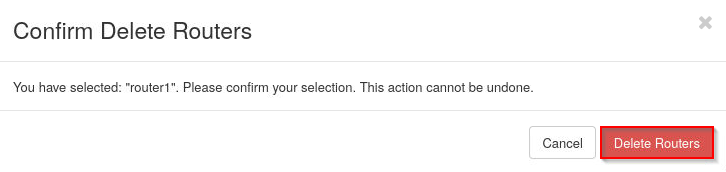
\includegraphics[width=\linewidth]{images/part1/step5.png}
        \end{center}
    \end{labstep}

    \begin{labstep}
        In previous labs, you disconnected routers from their subnets by using a \textbf{for} loop to iterate over interface IDs.
        In this lab, you will instead identify the connected subnets by name before disconnecting them.
        To begin, list the details of \textbf{router1} to see which subnets it is connected to.
        \begin{lstlisting}
            [ubuntu@workstation (keystone-admin)]:~$ openstack router show router1
        \end{lstlisting}

        \begin{center}
            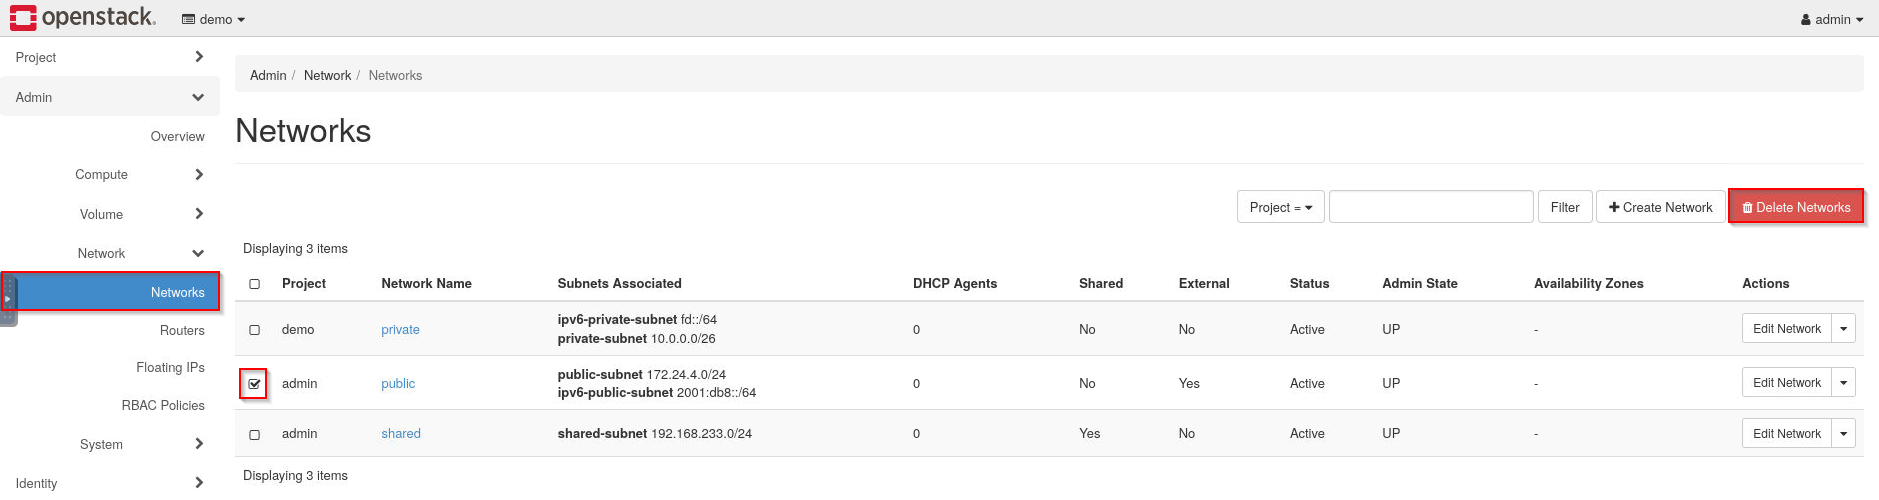
\includegraphics[width=\linewidth]{images/part1/step6.png}
        \end{center}
    \end{labstep}

    \begin{labstep}
        List the subnets to see the which names are mapped to the IDs from the previous step.
        \begin{lstlisting}
            [ubuntu@workstation (keystone-admin)]:~$ openstack subnet list
        \end{lstlisting}

        \begin{center}
            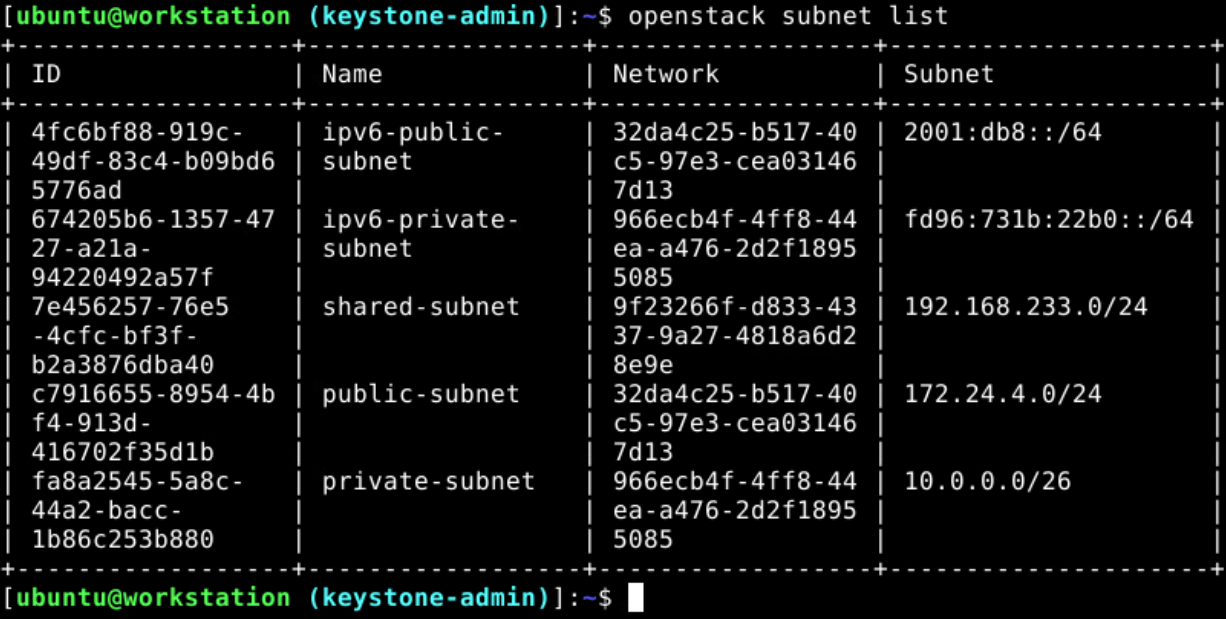
\includegraphics[width=\linewidth]{images/part1/step7.png}
        \end{center}
    \end{labstep}

    \begin{labstep}
        By matching the names and IDs, you can see that the router is connected to the \textbf{private-subnet} and \textbf{ipv6-private-subnet} subnets.
        Remove \textbf{private-subnet} subnet from \textbf{router1}.
        \begin{lstlisting}
            [ubuntu@workstation (keystone-admin)]:~$ openstack router remove subnet \
            > router1 \
            > private-subnet
        \end{lstlisting}

        \begin{center}
            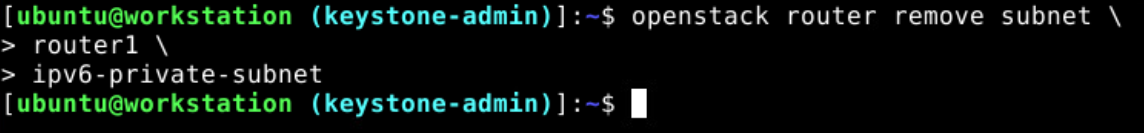
\includegraphics[width=\linewidth]{images/part1/step8.png}
        \end{center}
    \end{labstep}

    \begin{labstep}
        Now, remove \textbf{ipv6-private-subnet} from \textbf{router1}.
        \begin{lstlisting}
            [ubuntu@workstation (keystone-admin)]:~$ openstack router remove subnet \
            > router1 \
            > ipv6-private-subnet
        \end{lstlisting}

        \begin{center}
            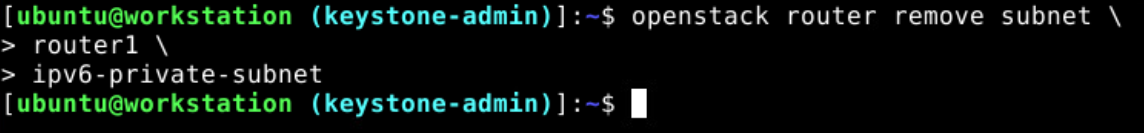
\includegraphics[width=\linewidth]{images/part1/step9.png}
        \end{center}
    \end{labstep}

    \begin{labstep}
        Now, the router can be deleted.
        Delete \textbf{router1}.
        \begin{lstlisting}
            [ubuntu@workstation (keystone-admin)]:~$ openstack router delete router1
        \end{lstlisting}

        \begin{center}
            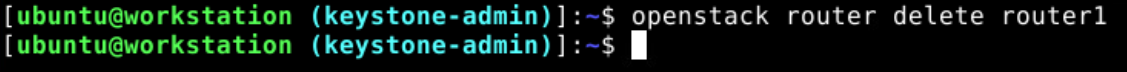
\includegraphics[width=\linewidth]{images/part1/step10.png}
        \end{center}
    \end{labstep}

    \begin{labstep}
        List the details of the available networks and find which one is external.
        The \textbf{--long} option adds several columns to the tabular output of the command, including the \textbf{Router Type} column, which shows whether the router is internal or external.
        We will limit the output to just the \textbf{Name} and \textbf{Router Type} columns.
        \begin{lstlisting}
            [ubuntu@workstation (keystone-admin)]:~$ openstack network list \
            > --long \
            > -c Name \
            > -c "Router Type"
        \end{lstlisting}

        \begin{center}
            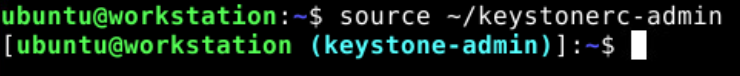
\includegraphics[width=\linewidth]{images/part1/step11.png}
        \end{center}
    \end{labstep}

    \begin{tipbox}
        In most terminal commands, arguments that contain spaces must be enclosed in quotation marks so that the shell treats them as a single value.
        In this case, \textbf{``Router~Type''} must be quoted to be interpreted correctly.
    \end{tipbox}

    \begin{labstep}
        The output of the previous step shows that \textbf{public} is the external network.
        Delete the \textbf{public} network.
        \begin{lstlisting}
            [ubuntu@workstation (keystone-admin)]:~$ openstack network delete public
        \end{lstlisting}

        \begin{center}
            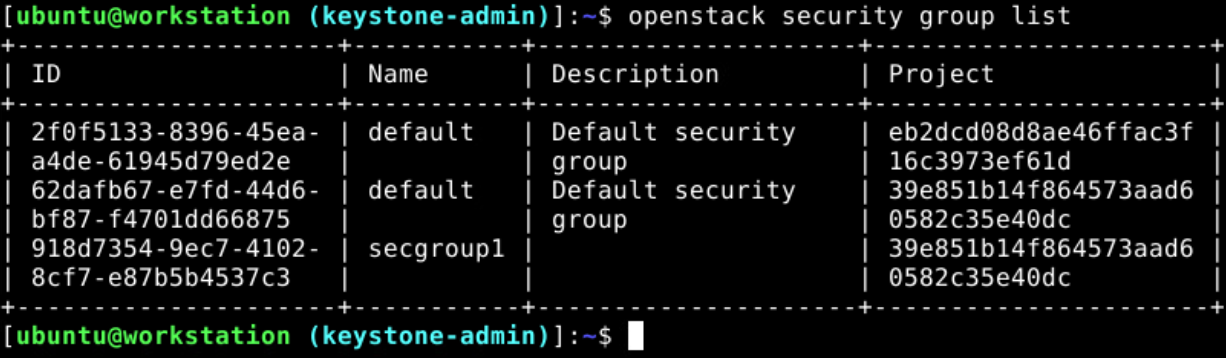
\includegraphics[width=\linewidth]{images/part1/step12.png}
        \end{center}
    \end{labstep}

    \begin{labstep}
        Now, we will create our own resources.
        First, create an external network named \textbf{extern-net}.
        Set the network type to \textbf{flat} and the physical network to \textbf{public}.
        Set the network as shared and external.
        \begin{lstlisting}
            [ubuntu@workstation (keystone-admin)]:~$ openstack network create \
            > --external \
            > --share \
            > --provider-network-type flat \
            > --provider-physical-network public \
            > extern-net
        \end{lstlisting}

        \begin{center}
            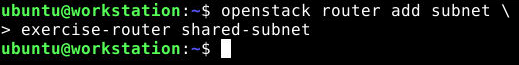
\includegraphics[width=\linewidth]{images/part1/step13.png}
        \end{center}
    \end{labstep}

    \begin{labstep}
        Create a subnet named \textbf{extern-subnet} in the \textbf{extern-net} network.
        Give the subnet a range of \textbf{172.25.250.60} to \textbf{172.25.250.80}.
        Disable DHCP services for the subnet and use the address \textbf{172.25.250.254} as the gateway as well as the DNS name server.
        \begin{lstlisting}
            [ubuntu@workstation (keystone-admin)]:~$ openstack subnet create \
            > --subnet-range 172.25.250.0/24 \
            > --no-dhcp \
            > --gateway 172.25.250.254 \
            > --dns-nameserver 172.25.250.254 \
            > --allocation-pool start=172.25.250.60,end=172.25.250.80 \
            > --network extern-net \
            > extern-subnet
        \end{lstlisting}

        \begin{center}
            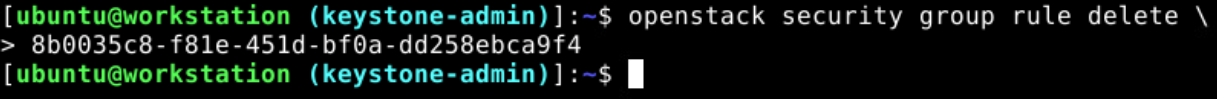
\includegraphics[width=\linewidth]{images/part1/step14.png}
        \end{center}
    \end{labstep}

    \begin{labstep}
        List the floating IPs to make sure none are already allocated.
        The list should be empty.
        \begin{lstlisting}
            [ubuntu@workstation (keystone-admin)]:~$ openstack floating ip list
        \end{lstlisting}

        \begin{center}
            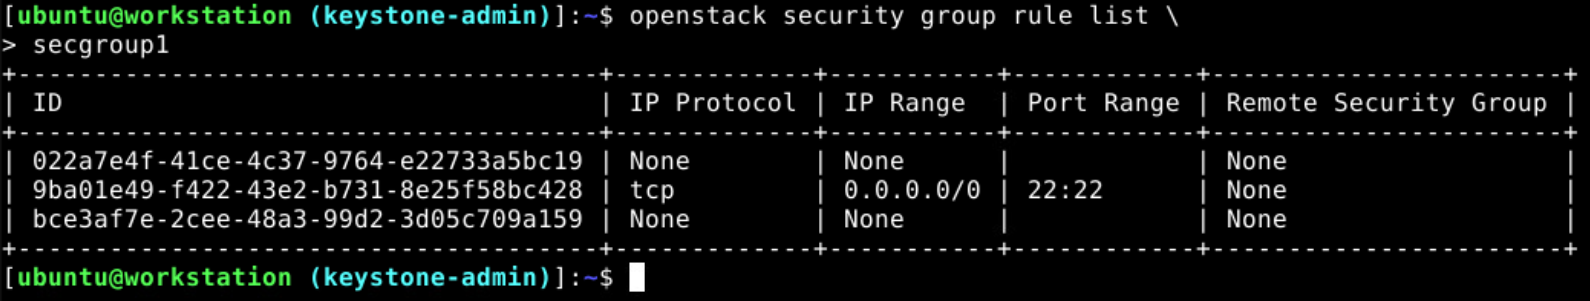
\includegraphics[width=\linewidth]{images/part1/step15.png}
        \end{center}
    \end{labstep}

    \begin{labstep}
        From the floating IP pool in the \textbf{extern-net} network, create a floating IP.
        \begin{lstlisting}
            [ubuntu@workstation (keystone-admin)]:~$ openstack floating ip create extern-net
        \end{lstlisting}

        \begin{center}
            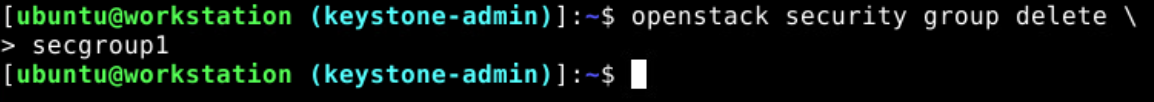
\includegraphics[width=\linewidth]{images/part1/step16.png}
        \end{center}
    \end{labstep}

    \begin{labstep}
        Create a router named \textbf{extern-router}.
        \begin{lstlisting}
            [ubuntu@workstation (keystone-admin)]:~$ openstack router create extern-router
        \end{lstlisting}

        \begin{center}
            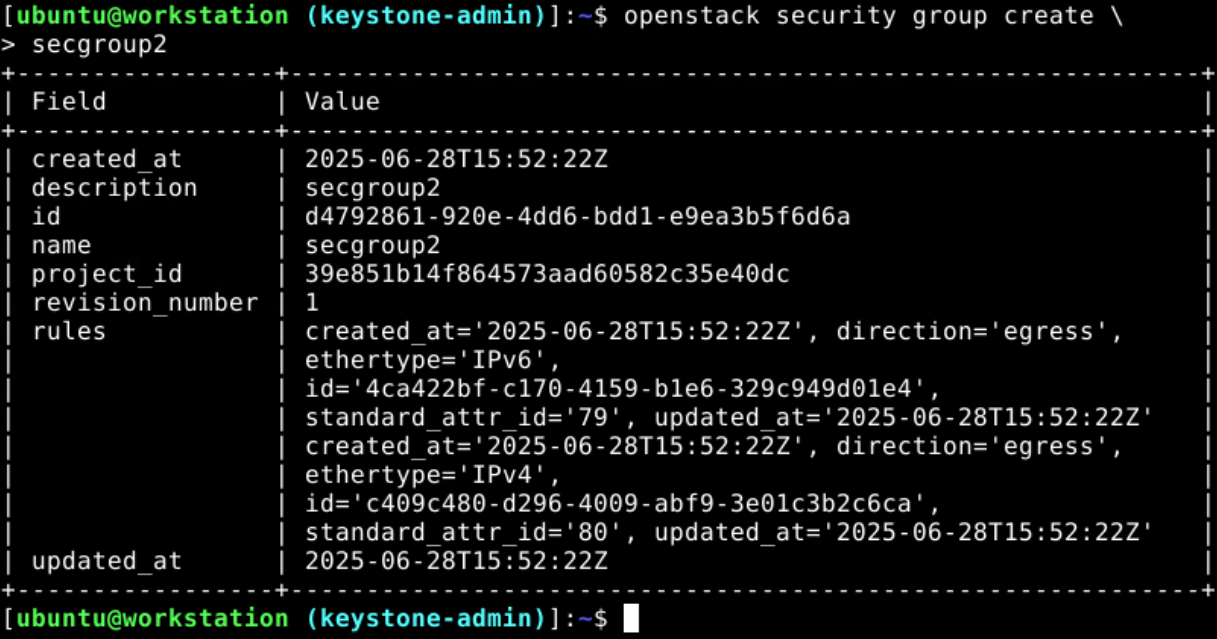
\includegraphics[width=\linewidth]{images/part1/step17.png}
        \end{center}
    \end{labstep}

    \begin{labstep}
        List the available subnets to see what the router can be connected to.
        \begin{lstlisting}
            [ubuntu@workstation (keystone-admin)]:~$ openstack subnet list
        \end{lstlisting}

        \begin{center}
            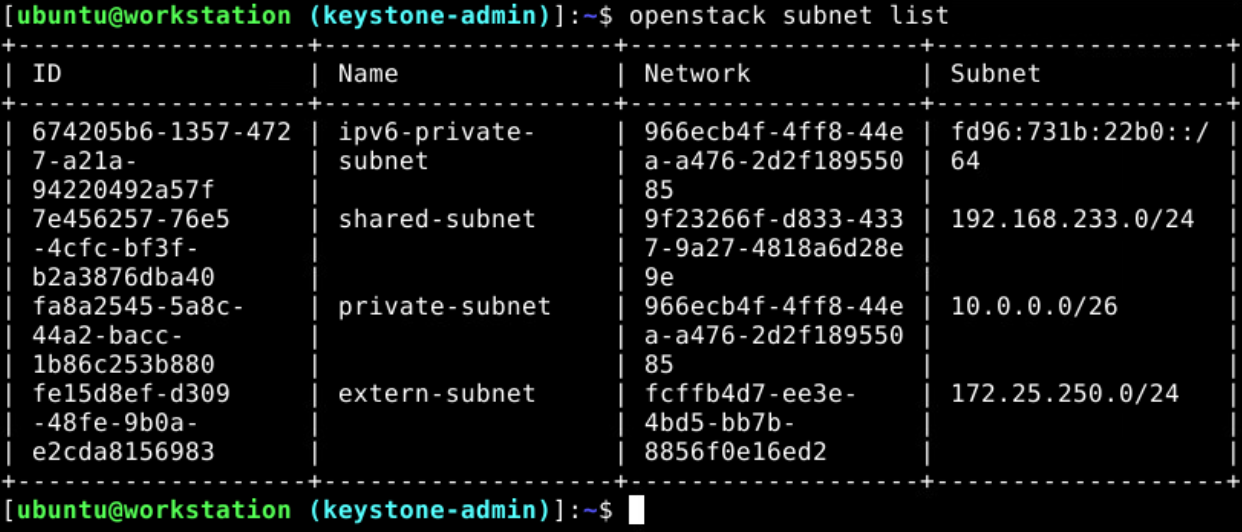
\includegraphics[width=\linewidth]{images/part1/step18.png}
        \end{center}
    \end{labstep}

    \begin{labstep}
        Connect the router to the \textbf{shared-subnet} subnet.
        \begin{lstlisting}
            [ubuntu@workstation (keystone-admin)]:~$ openstack router add subnet \
            > extern-router shared-subnet
        \end{lstlisting}

        \begin{center}
            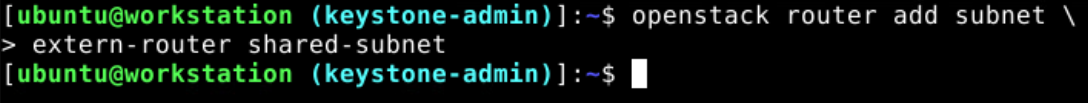
\includegraphics[width=\linewidth]{images/part1/step19.png}
        \end{center}
    \end{labstep}

    \begin{labstep}
        Set the \textbf{extern-net} network as the gateway for the router.
        \begin{lstlisting}
            [ubuntu@workstation (keystone-admin)]:~$ openstack router set \
            > --external-gateway extern-net \
            > extern-router
        \end{lstlisting}

        \begin{center}
            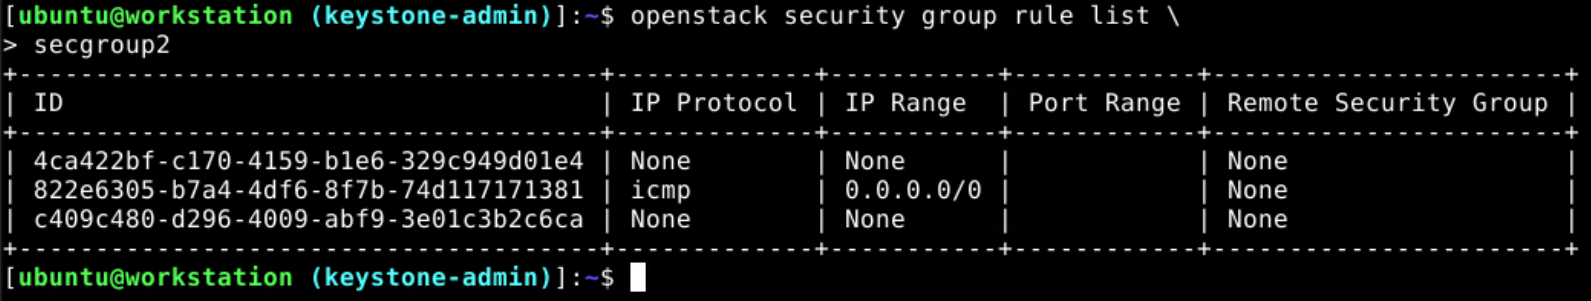
\includegraphics[width=\linewidth]{images/part1/step20.png}
        \end{center}
    \end{labstep}

    \begin{labstep}
        List the current key pairs to make sure there are not any already allocated.
        The list should be empty.
        \begin{lstlisting}
            [ubuntu@workstation (keystone-admin)]:~$ openstack keypair list
        \end{lstlisting}

        \begin{center}
            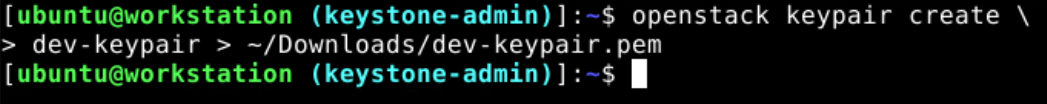
\includegraphics[width=\linewidth]{images/part1/step21.png}
        \end{center}
    \end{labstep}

    \begin{labstep}
        Create the key pair \textbf{dev-keypair} and save the private key to the file
        \textbf{\texttildemid/Downloads/dev-keypair.pem}.
        \begin{lstlisting}
            [ubuntu@workstation (keystone-admin)]:~$ openstack keypair create \
            > dev-keypair > ~/Downloads/dev-keypair.pem
        \end{lstlisting}

        \begin{center}
            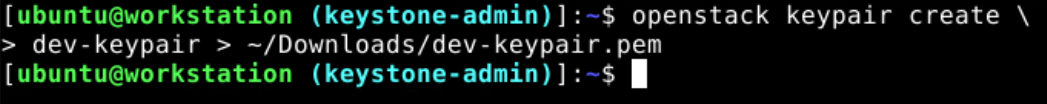
\includegraphics[width=\linewidth]{images/part1/step22.png}
        \end{center}
    \end{labstep}

    \begin{labstep}
        View the permission of the \textbf{~/Downloads/dev-keypair.pem} file.
        You can see that the \textbf{ubuntu} user has read and write privileges to the file, the \textbf{ubuntu} user group has read and write privileges to the file, and other users have read permissions to the file.
        However, this is a sensitive file, and only the \textbf{ubuntu} user should have any privileges to it.
        \begin{lstlisting}
            [ubuntu@workstation (keystone-admin)]:~$ ls -l ~/Downloads/dev-keypair.pem
        \end{lstlisting}

        \begin{center}
            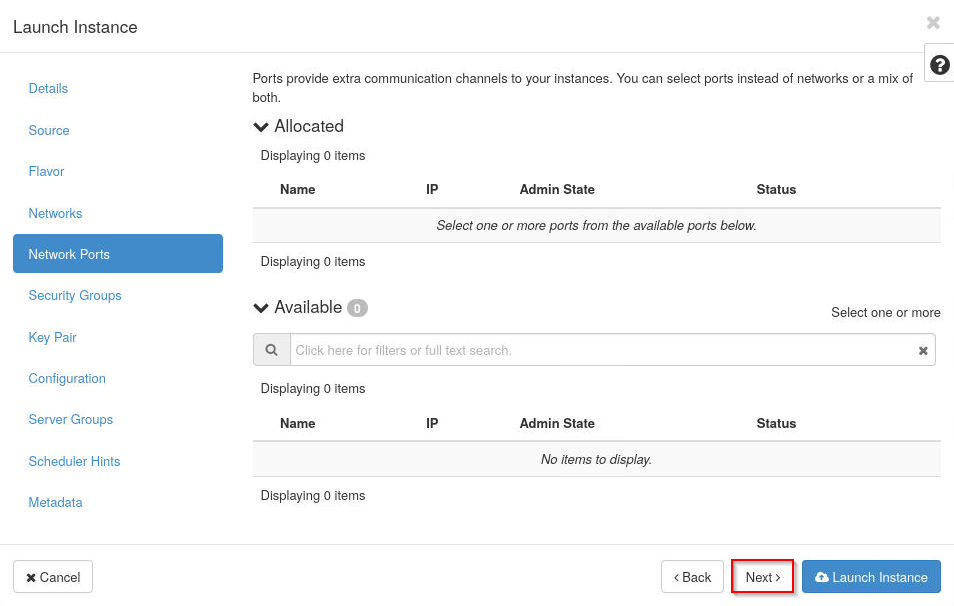
\includegraphics[width=\linewidth]{images/part1/step23.png}
        \end{center}
    \end{labstep}

    \begin{labstep}
        Use the \textbf{chmod} command with a mode of \textbf{600} to make it so that the \textbf{ubuntu} user has read/write permissions on the file, and groups and other users have no permissions to the file.
        \begin{lstlisting}
            [ubuntu@workstation (keystone-admin)]:~$ chmod 600 ~/Downloads/dev-keypair.pem
        \end{lstlisting}

        \begin{center}
            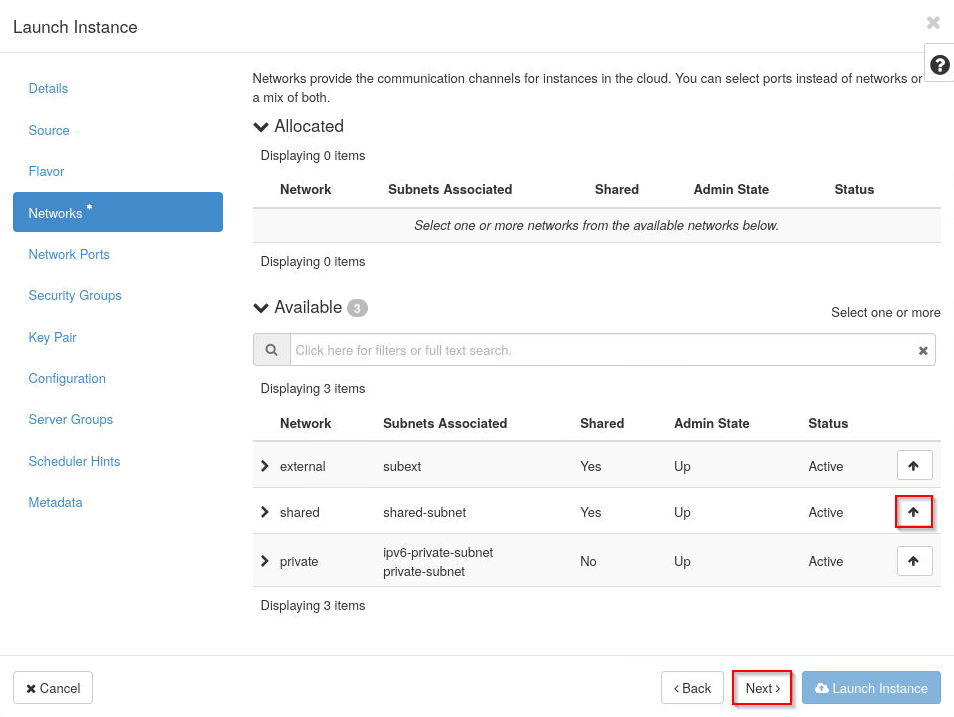
\includegraphics[width=\linewidth]{images/part1/step24.png}
        \end{center}
    \end{labstep}

    \begin{labstep}
        List the permissions again to ensure that the change took effect.
        \begin{lstlisting}
            [ubuntu@workstation (keystone-admin)]:~$ ls -l ~/Downloads/dev-keypair.pem
        \end{lstlisting}

        \begin{center}
            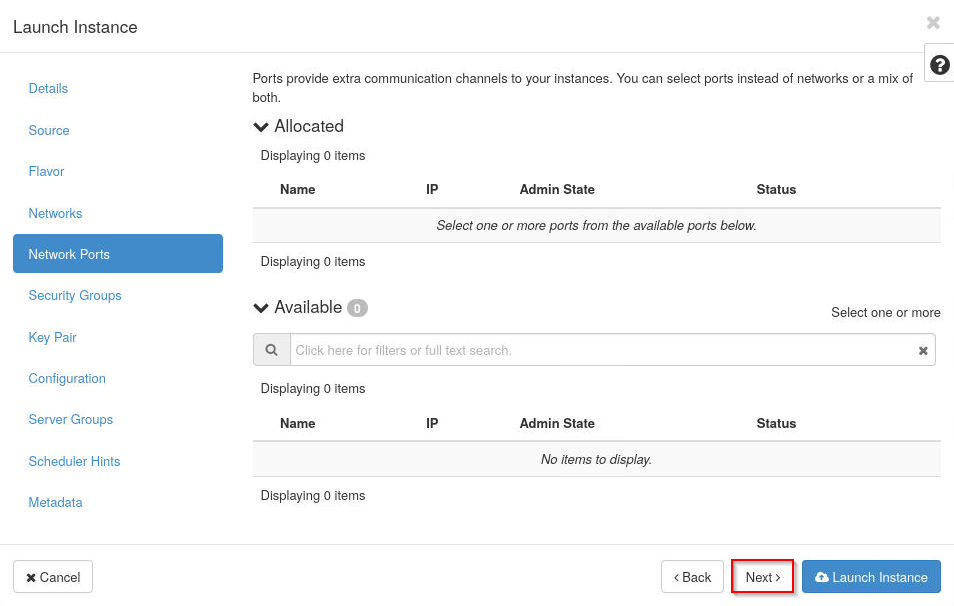
\includegraphics[width=\linewidth]{images/part1/step25.png}
        \end{center}
    \end{labstep}

    \begin{labstep}
        Create the \textbf{dev-secgroup} security group.
        \begin{lstlisting}
            [ubuntu@workstation (keystone-admin)]:~$ openstack security group create \
            > dev-secgroup
        \end{lstlisting}

        \begin{center}
            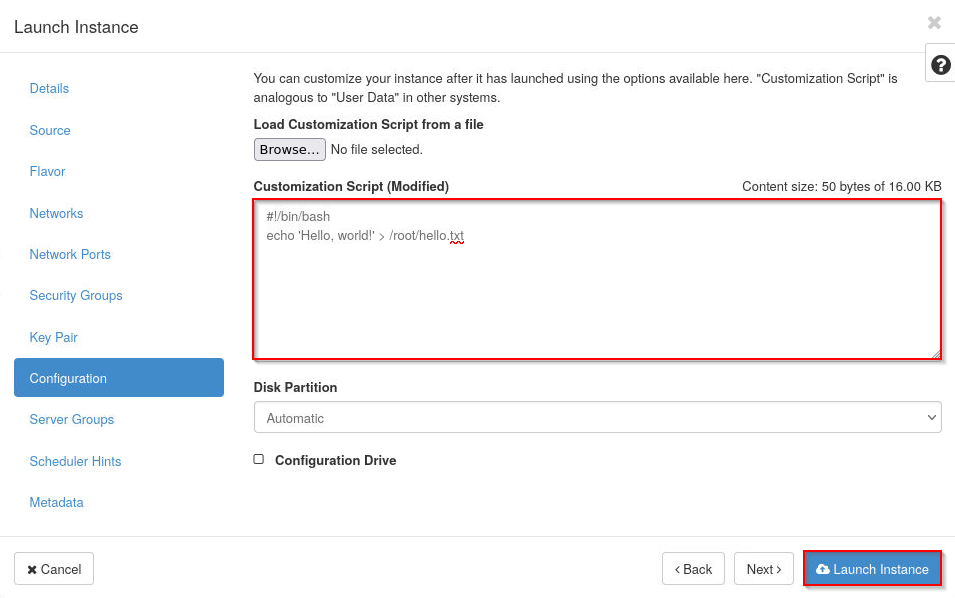
\includegraphics[width=\linewidth]{images/part1/step26.png}
        \end{center}
    \end{labstep}

    \begin{labstep}
        List the default security group rules.
        \begin{lstlisting}
            [ubuntu@workstation (keystone-admin)]:~$ openstack security group rule list \
            > dev-secgroup
        \end{lstlisting}

        \begin{center}
            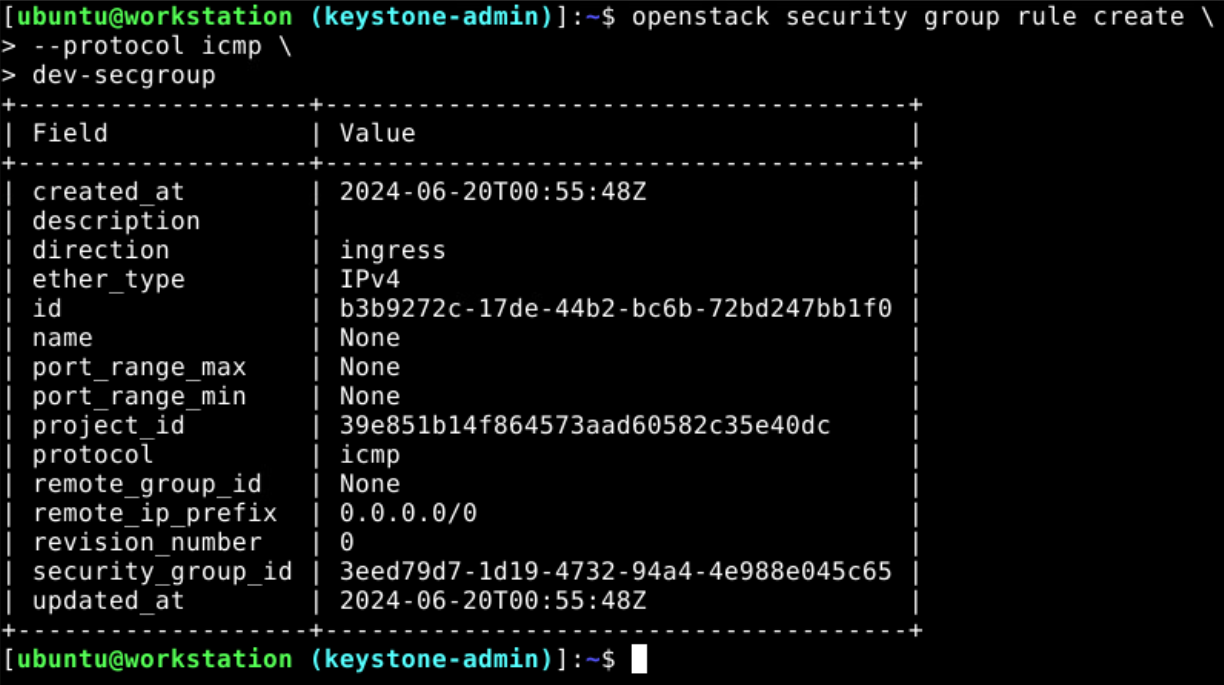
\includegraphics[width=\linewidth]{images/part1/step27.png}
        \end{center}
    \end{labstep}

    \begin{tipbox}
        You can verify that the default rules allow any outgoing traffic over IPv4 or IPv6 with this command:
        \begin{lstlisting}
            openstack security group rule show <rule-id>
        \end{lstlisting}
    \end{tipbox}

    \begin{labstep}
        Add a security rule in the \textbf{dev-secgroup} security group to allow remote ICMP traffic.
        \begin{lstlisting}
            [ubuntu@workstation (keystone-admin)]:~$ openstack security group rule create \
            > --protocol icmp \
            > dev-secgroup
        \end{lstlisting}

        \begin{center}
            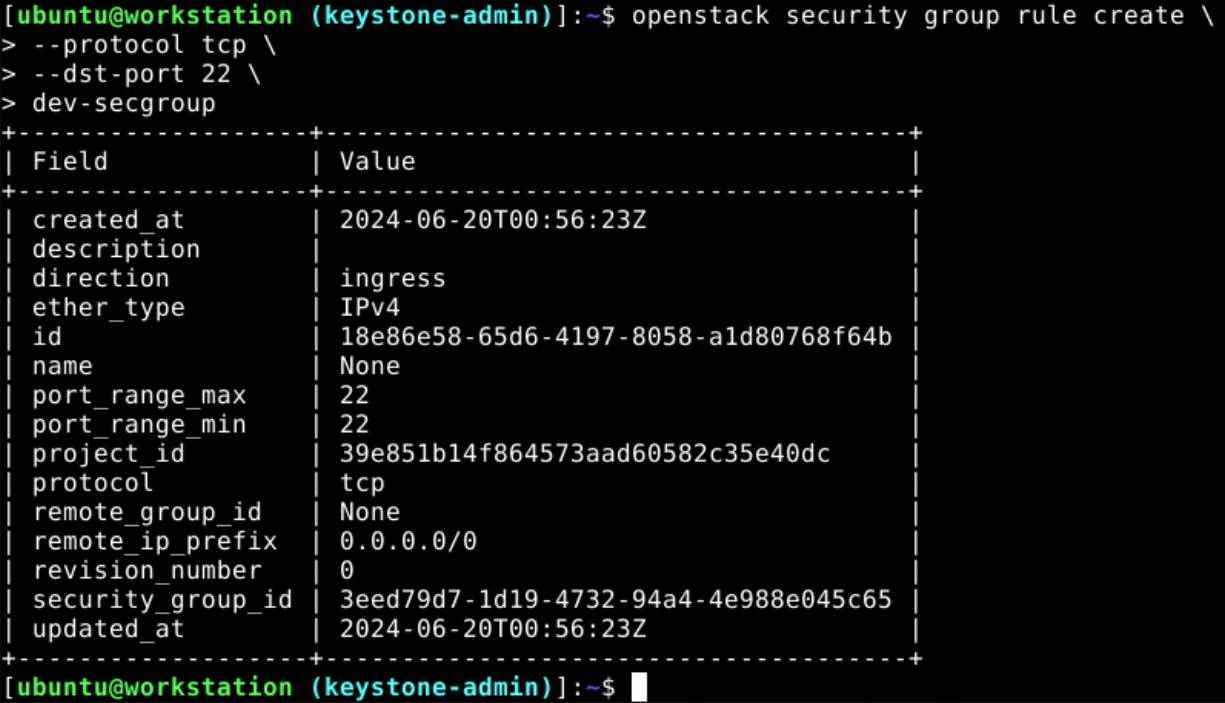
\includegraphics[width=\linewidth]{images/part1/step28.png}
        \end{center}
    \end{labstep}

    \begin{labstep}
        Add another security rule to allow remote connection using SSH on the default port 22.
        \begin{lstlisting}
            [ubuntu@workstation (keystone-admin)]:~$ openstack security group rule create \
            > --protocol tcp \
            > --dst-port 22 \
            > dev-secgroup
        \end{lstlisting}

        \begin{center}
            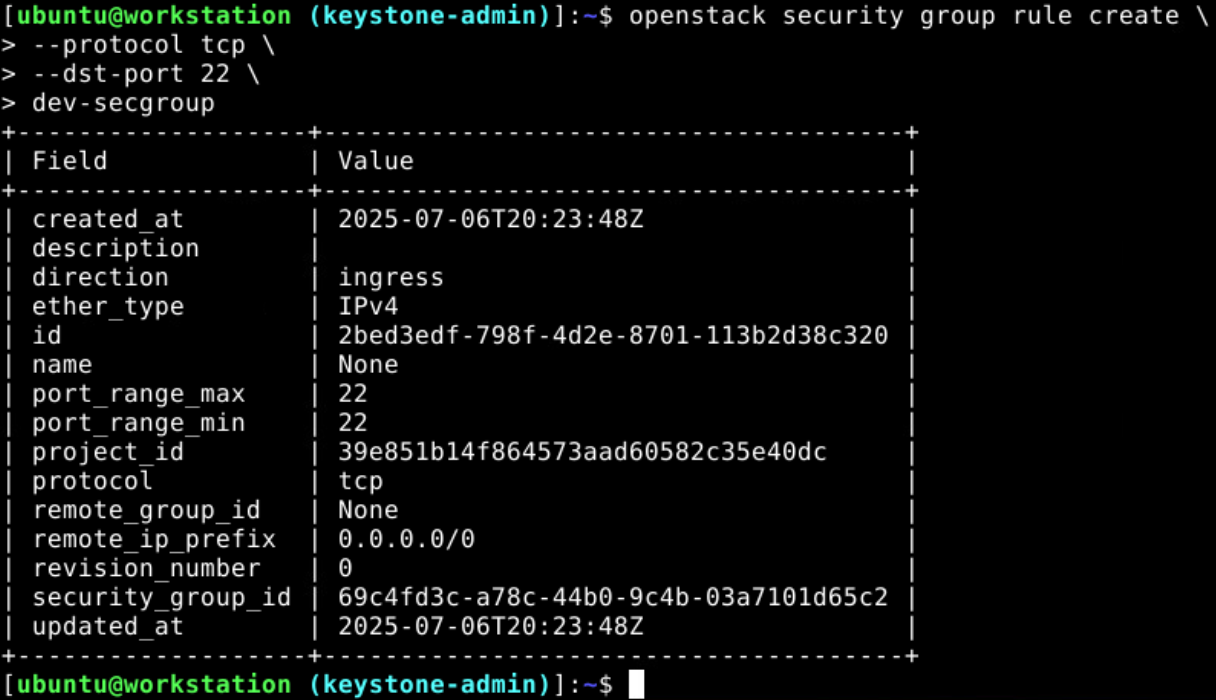
\includegraphics[width=\linewidth]{images/part1/step29.png}
        \end{center}
    \end{labstep}

    \begin{labstep}
        List the security group rules again to see that the new rules have taken effect.
        \begin{lstlisting}
            [ubuntu@workstation (keystone-admin)]:~$ openstack security group rule list \
            > dev-secgroup
        \end{lstlisting}

        \begin{center}
            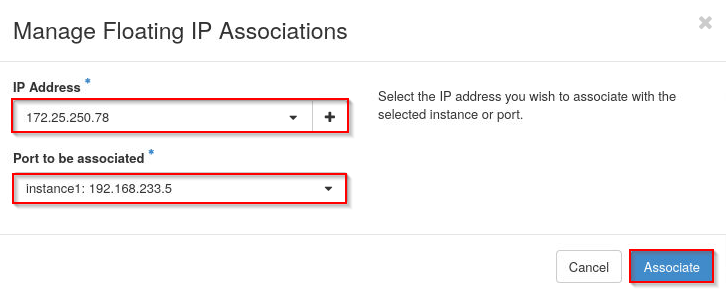
\includegraphics[width=\linewidth]{images/part1/step30.png}
        \end{center}
    \end{labstep}

    \begin{labstep}
        Close the terminal window, and continue to the next task.
    \end{labstep}
\end{enumerate}

%%%%%%%%%%%
% Section 2
%%%%%%%%%%%
\section{Creating a Customized Instance with the Horizon Dashboard}\label{sec:creating-a-customized-instance-with-the-horizon-dashboard}
In this task, you will create a customized instance with the Horizon Dashboard and log into the instance to verify that the customization took effect.

\begin{enumerate}
    \begin{labstep}
        Open the web browser and navigate to \textbf{192.168.1.20}.
        Log into the dashboard as \textbf{admin} with the password \textbf{secret}.
    \end{labstep}

    \begin{labstep}
        Make sure the \textbf{demo} project is selected.
        Navigate to \textbf{Project $>$ Compute $>$ Instances}, and click \textbf{Launch Instance}.

        \begin{center}
            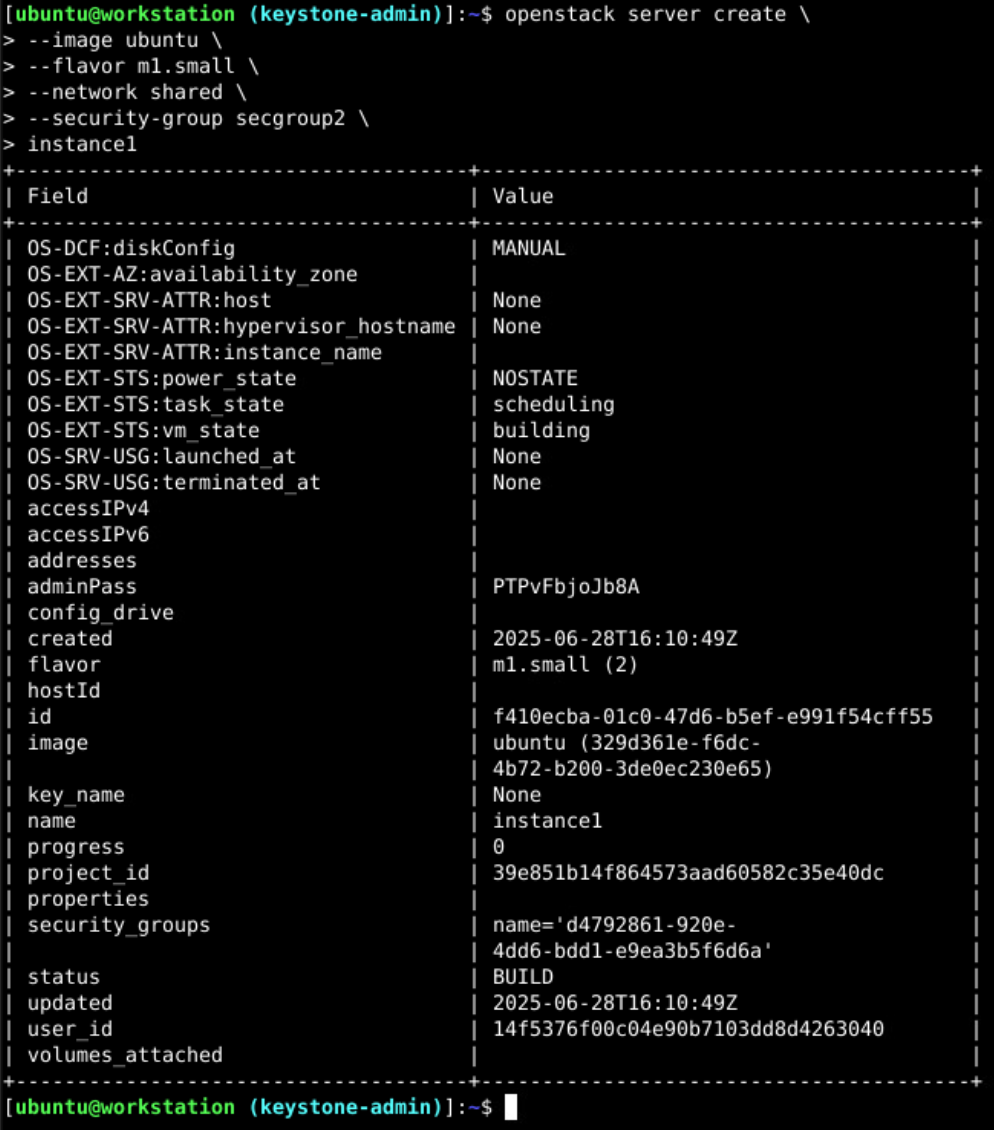
\includegraphics[width=\linewidth]{images/part2/step2.png}
        \end{center}
    \end{labstep}

    \begin{labstep}
        In the \textit{Details} tab, enter \textbf{instance1} in the \textit{Instance Name} field and click \textbf{Next}.

        \begin{center}
            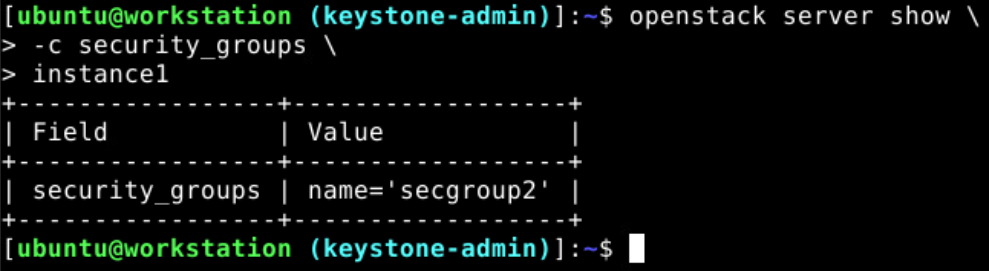
\includegraphics[width=\linewidth]{images/part2/step3.png}
        \end{center}
    \end{labstep}

    \begin{labstep}
        In the \textit{Source} tab, make sure \textbf{Image} is selected in the \textit{Select Boot Source} dropdown and click \textbf{No} under \textit{Create New Volume}.
        Select the \textbf{ubuntu} image by clicking the $\uparrow$ symbol in the same row.
        Click \textbf{Next}.

        \begin{center}
            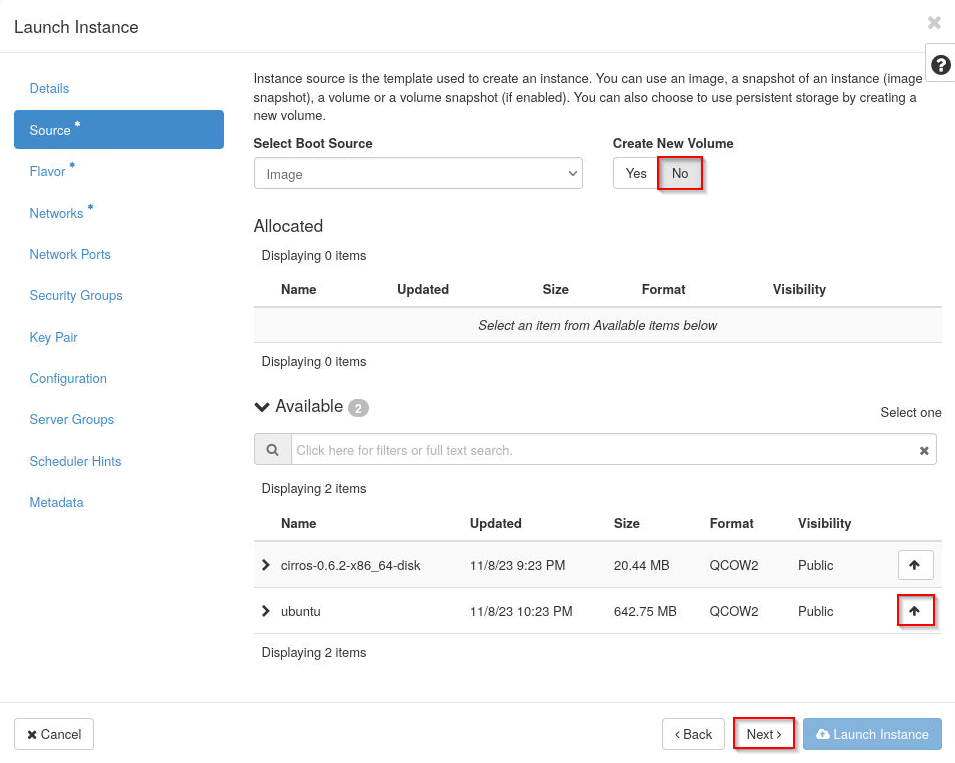
\includegraphics[width=\linewidth]{images/part2/step4.png}
        \end{center}
    \end{labstep}

    \begin{stopbox}
        Before proceeding to the next step, confirm that \textbf{ubuntu} appears underneath the \textit{Allocated} section.
    \end{stopbox}

    \begin{labstep}
        In the \textit{Flavor} tab, click the $\uparrow$ symbol in the same row as \textbf{m1.small}
        Click \textbf{Next}.

        \begin{center}
            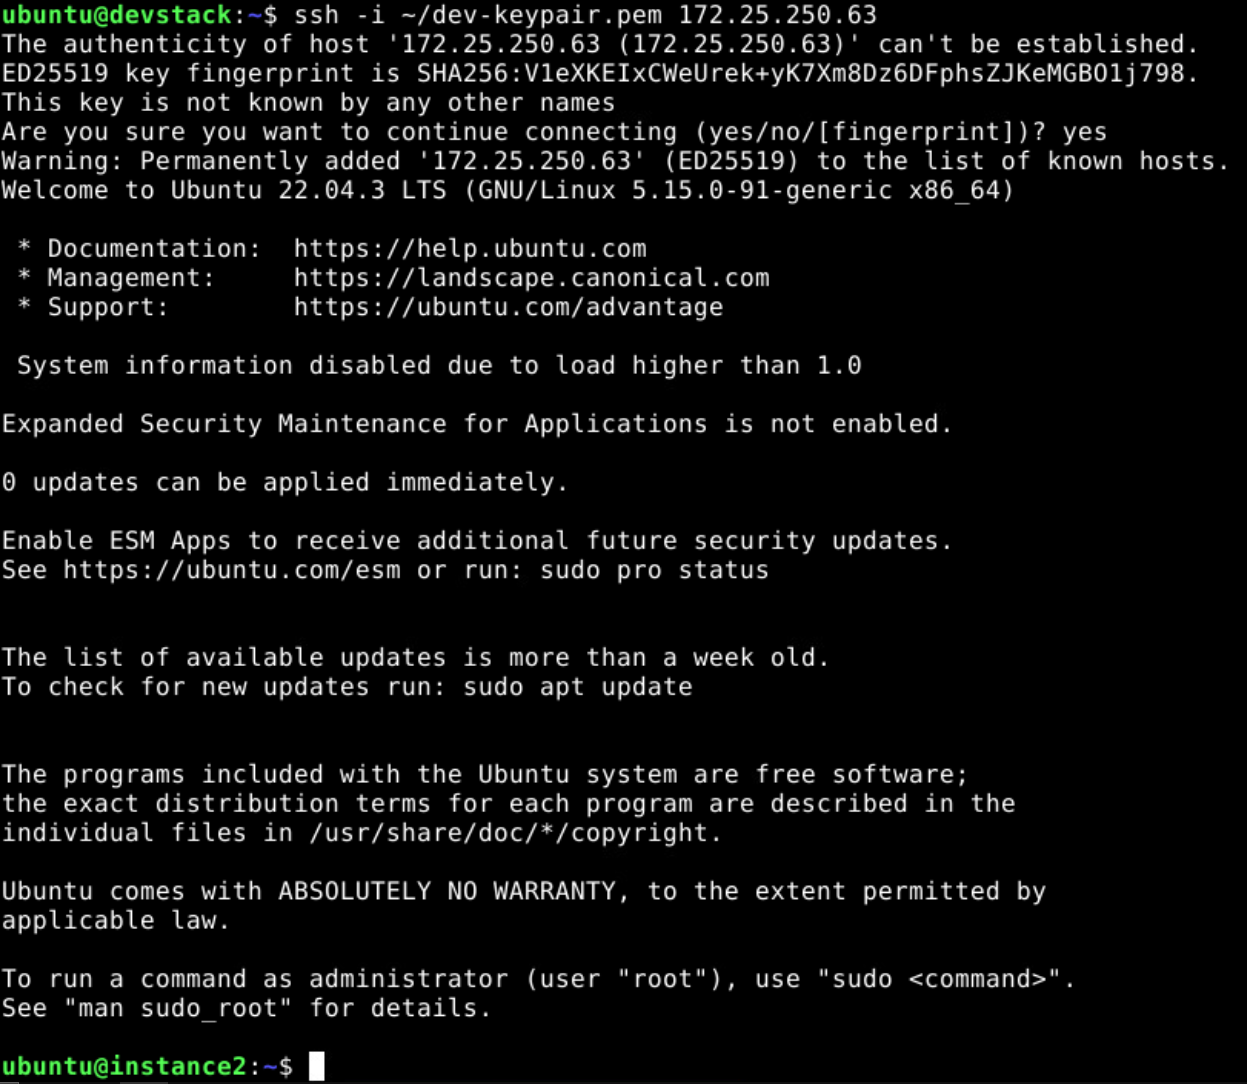
\includegraphics[width=\linewidth]{images/part2/step5.png}
        \end{center}
    \end{labstep}

    \begin{stopbox}
        Before proceeding to the next step, confirm that \textbf{m1.small} appears underneath the \textit{Allocated} section.
    \end{stopbox}

    \begin{labstep}
        In the \textit{Networks} tab, click the $\uparrow$ symbol in the same row as \textbf{shared}.
        Click \textbf{Next}.

        \begin{center}
            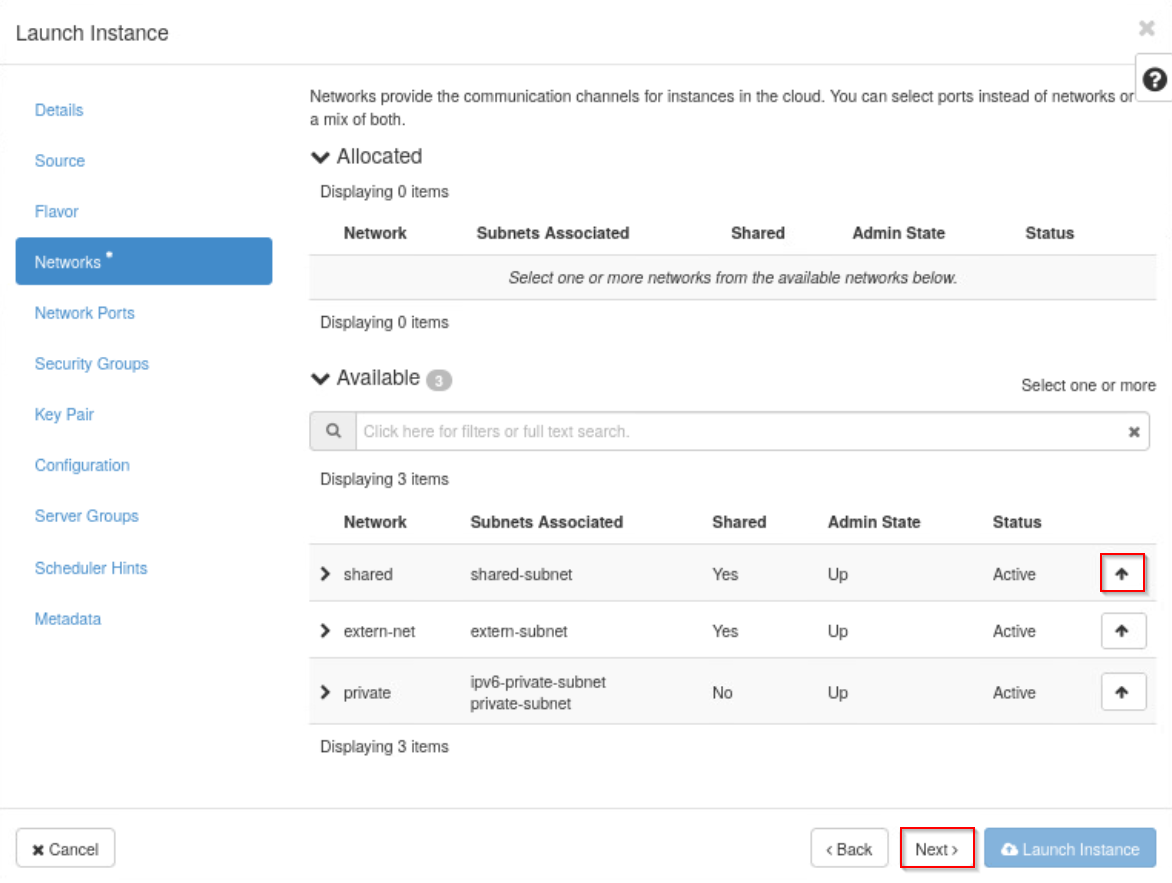
\includegraphics[width=\linewidth]{images/part2/step6.png}
        \end{center}
    \end{labstep}

    \begin{stopbox}
        Before proceeding to the next step, confirm that \textbf{shared} appears underneath the \textit{Allocated} section.
    \end{stopbox}

    \begin{labstep}
        In the \textit{Network Ports} tab, click \textbf{Next}.

        \begin{center}
            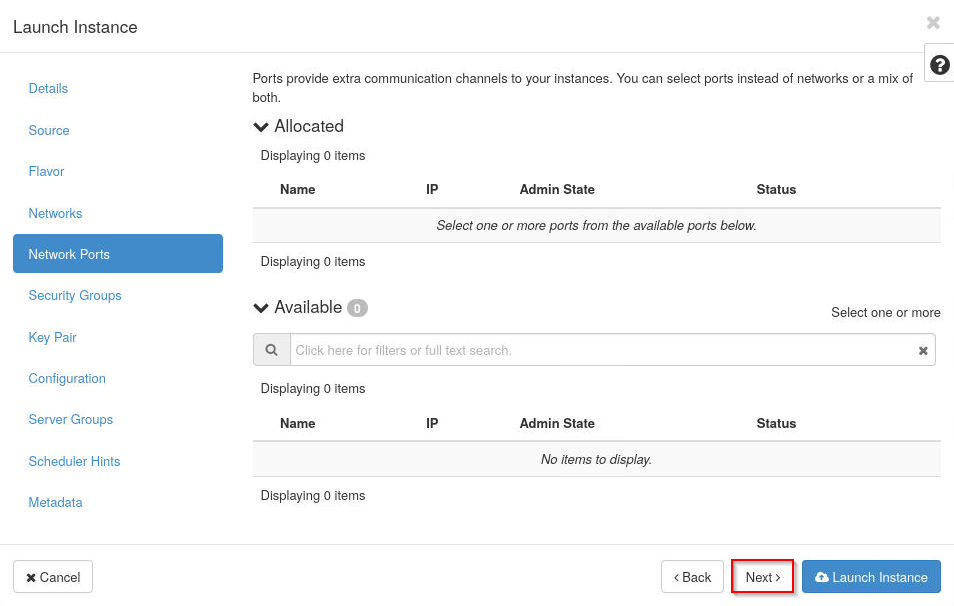
\includegraphics[width=\linewidth]{images/part2/step7.png}
        \end{center}
    \end{labstep}

    \begin{labstep}
        In the \textit{Security Groups} tab, click the $\downarrow$ symbol in the same row as \textbf{default}, and click the $\uparrow$ symbol in the same row as \textbf{dev-secgroup}.
        Click \textbf{Next}.

        \begin{center}
            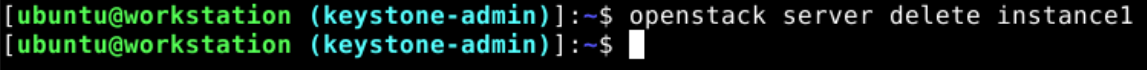
\includegraphics[width=\linewidth]{images/part2/step8.png}
        \end{center}
    \end{labstep}

    \begin{stopbox}
        Before proceeding to the next step, confirm that only \textbf{dev-secgroup} appears underneath the \textit{Allocated} section.
    \end{stopbox}

    \begin{labstep}
        In the \textit{Key Pair} tab, ensure that the key pair \textbf{dev-keypair} has been selected and is underneath the \textit{Allocated} section.
        Click \textbf{Next}.

        \begin{center}
            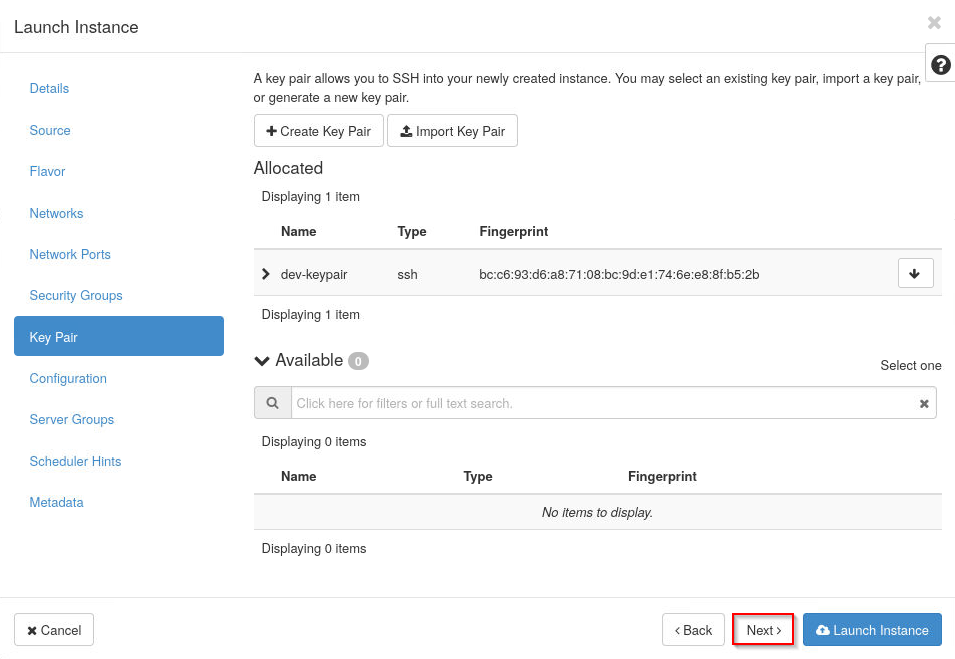
\includegraphics[width=\linewidth]{images/part2/step9.png}
        \end{center}
    \end{labstep}

    \begin{labstep}
        In the \textit{Configuration} tab, populate the \textbf{Customization Script} field with the content below.
        Once finished, click \textbf{Launch Instance}.
        \begin{lstlisting}
            #!/bin/bash
            echo 'Hello, world!' > /root/hello.txt
        \end{lstlisting}

        \begin{center}
            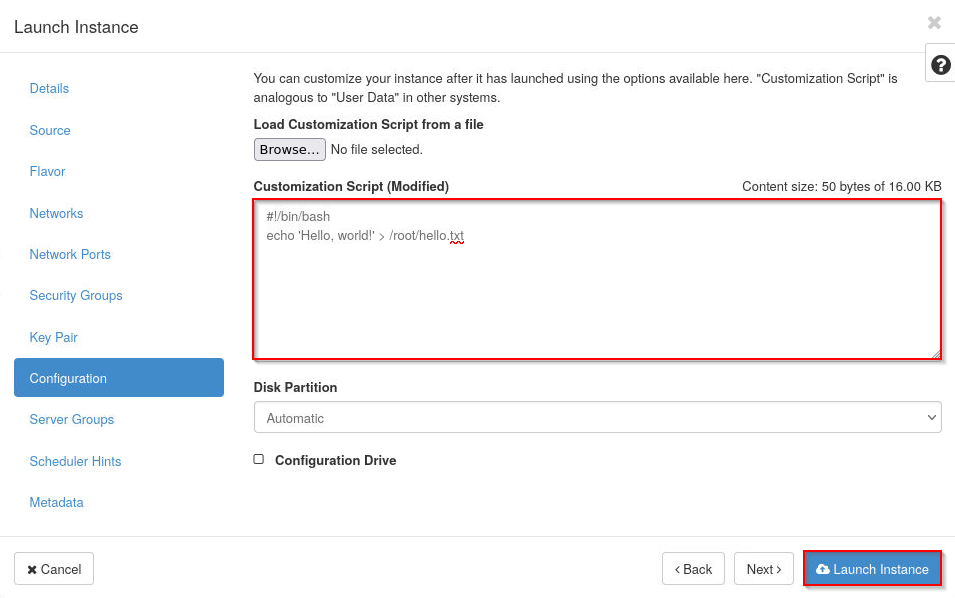
\includegraphics[width=\linewidth]{images/part2/step10.png}
        \end{center}
    \end{labstep}

    \begin{tipbox}
        A customization script can be used to perform many commands automatically upon instance creation, such as installing packages, configuring a host name, etc.
        The simple script above is just an example.
    \end{tipbox}

    \begin{labstep}
        Once the status for \textbf{instance1} is \textbf{Active}, attach a floating IP address to it.
        Select \textbf{Associate Floating IP} from the dropdown menu next to \textbf{Create Snapshot} in the row for the instance.

        \begin{center}
            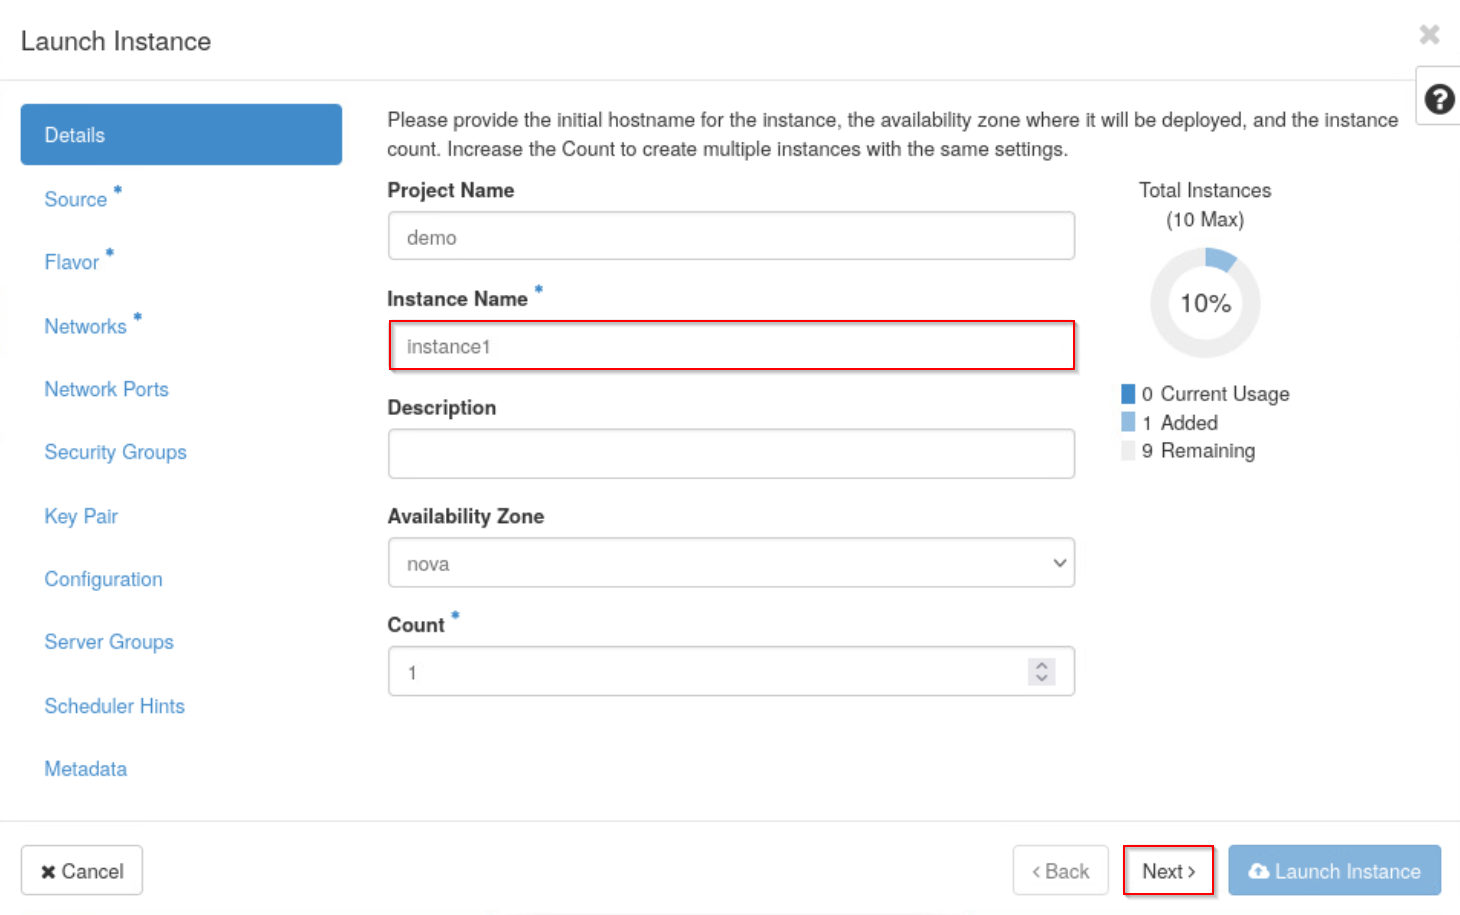
\includegraphics[width=\linewidth]{images/part2/step11.png}
        \end{center}
    \end{labstep}

    \begin{labstep}
        Select any one of the IP addresses from the \textit{IP Address} dropdown and select \textbf{instance1: 192.168.233.XYZ} as the \textit{Port to be associated}.
        Click \textbf{Associate}.

        \begin{center}
            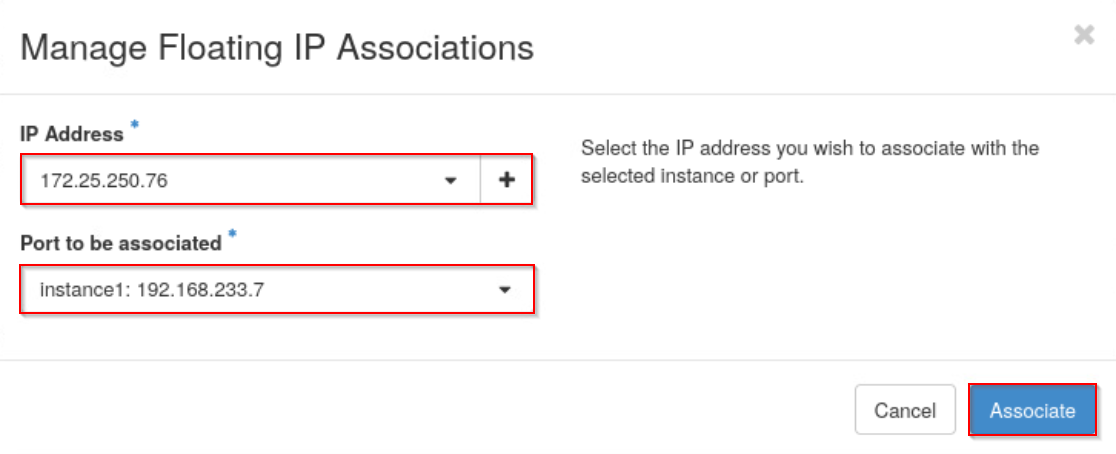
\includegraphics[width=\linewidth]{images/part2/step12.png}
        \end{center}
    \end{labstep}

    \begin{labstep}
        To verify that the customization script worked, first click \textbf{instance1} under the \textit{Instance Name} column, then navigate to the \textit{Console} tab if you are not directed there automatically.
        Click the \textbf{Click here to show only the console} link.
        Log into the instance as \textbf{root} with the password \textbf{secret}.

        \begin{center}
            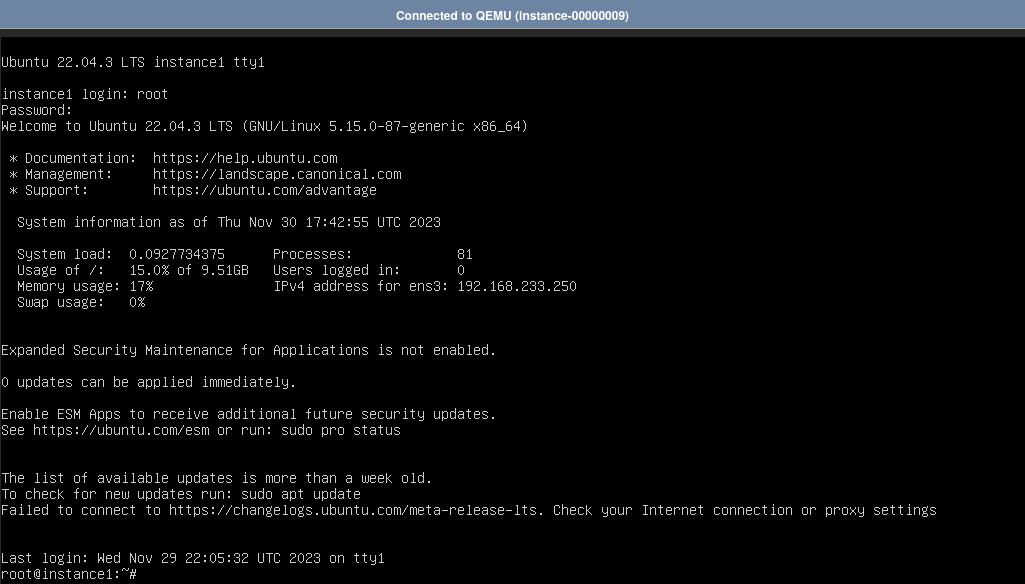
\includegraphics[width=\linewidth]{images/part2/step13.png}
        \end{center}
    \end{labstep}

    \begin{notebox}
        Be patient for the login prompt.
        Even if OpenStack reports the instance to be active, it may still take several minutes to fully launch and present the login prompt.
    \end{notebox}

    \begin{labstep}
        Check \textbf{/var/log/cloud-init.log} to confirm that \textbf{cloud-init} ran.
        Use the \textbf{tail} command to print the last 10 lines of the log.
        \begin{lstlisting}
            root@instance1:~# sudo tail /var/log/cloud-init.log
        \end{lstlisting}

        \begin{center}
            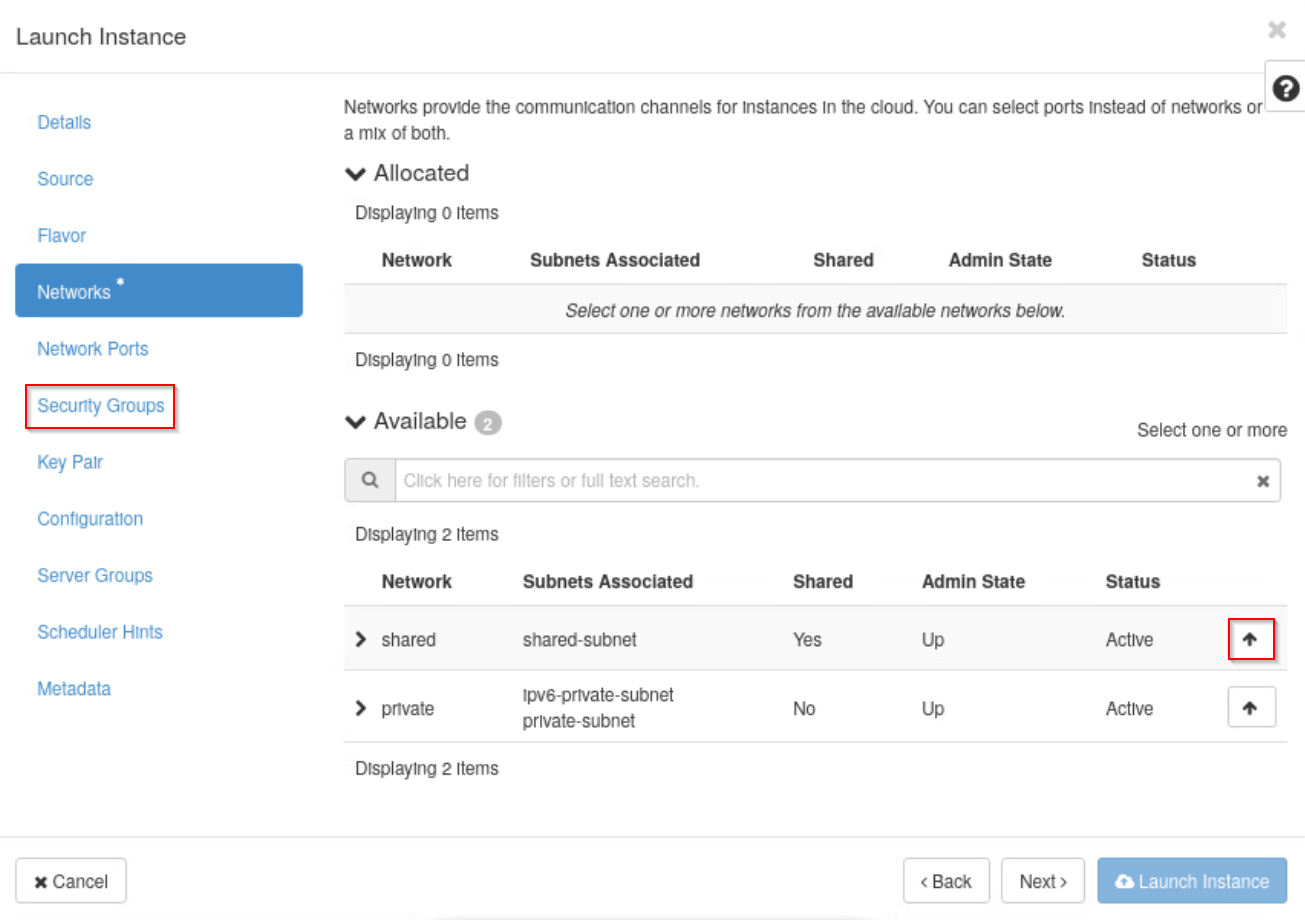
\includegraphics[width=\linewidth]{images/part2/step14.png}
        \end{center}
    \end{labstep}

    \begin{labstep}
        Ensure that the \textbf{/root/hello.txt} file exists and has the correct content.
        \begin{lstlisting}
            root@instance1:~# cat /root/hello.txt
        \end{lstlisting}

        \begin{center}
            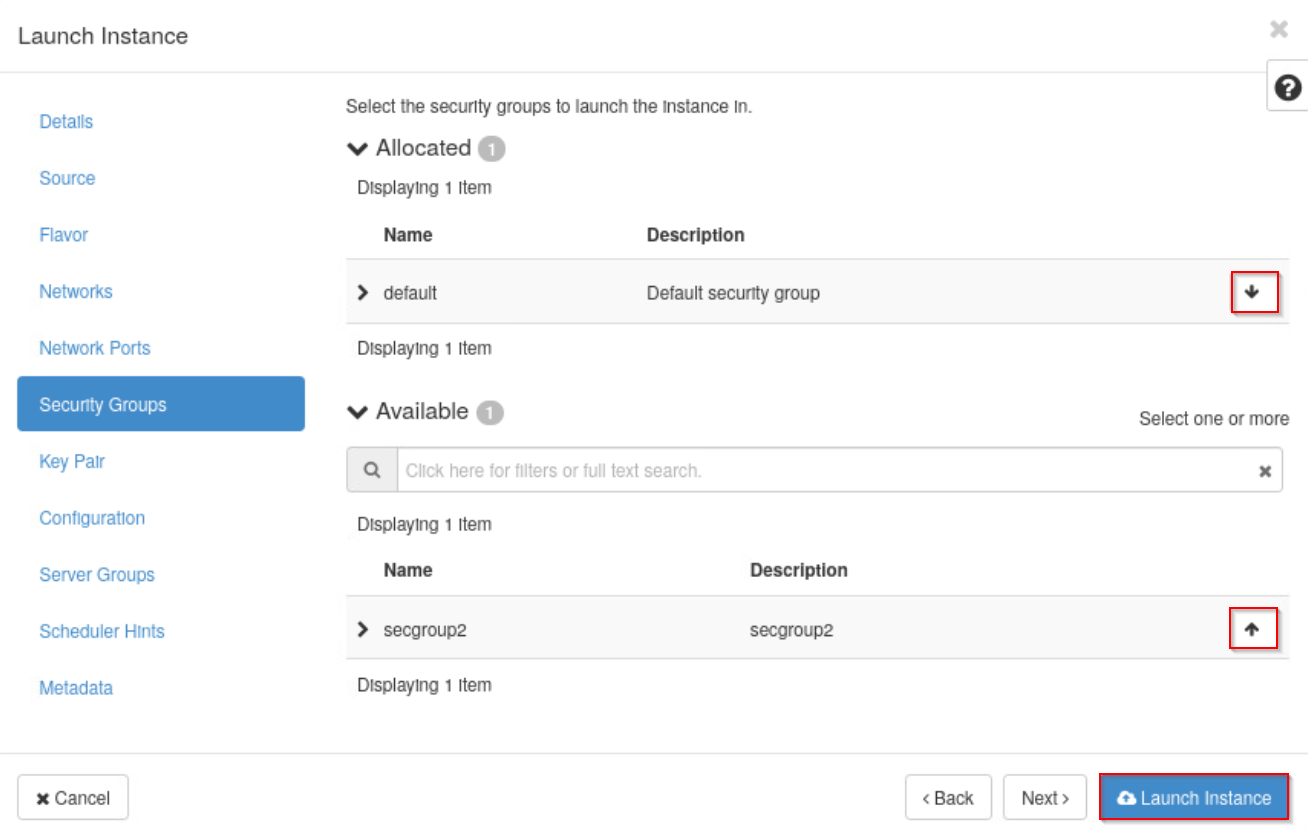
\includegraphics[width=\linewidth]{images/part2/step15.png}
        \end{center}
    \end{labstep}

    \begin{labstep}
        Close the tab with the terminal window and navigate back to \textbf{Project $>$ Compute $>$ Instances} if you are not already on that page.
        We are finished with this instance and will create another one in the next section.
        Select the checkbox next to \textbf{instance1} and click \textbf{Delete Instances}.

        \begin{center}
            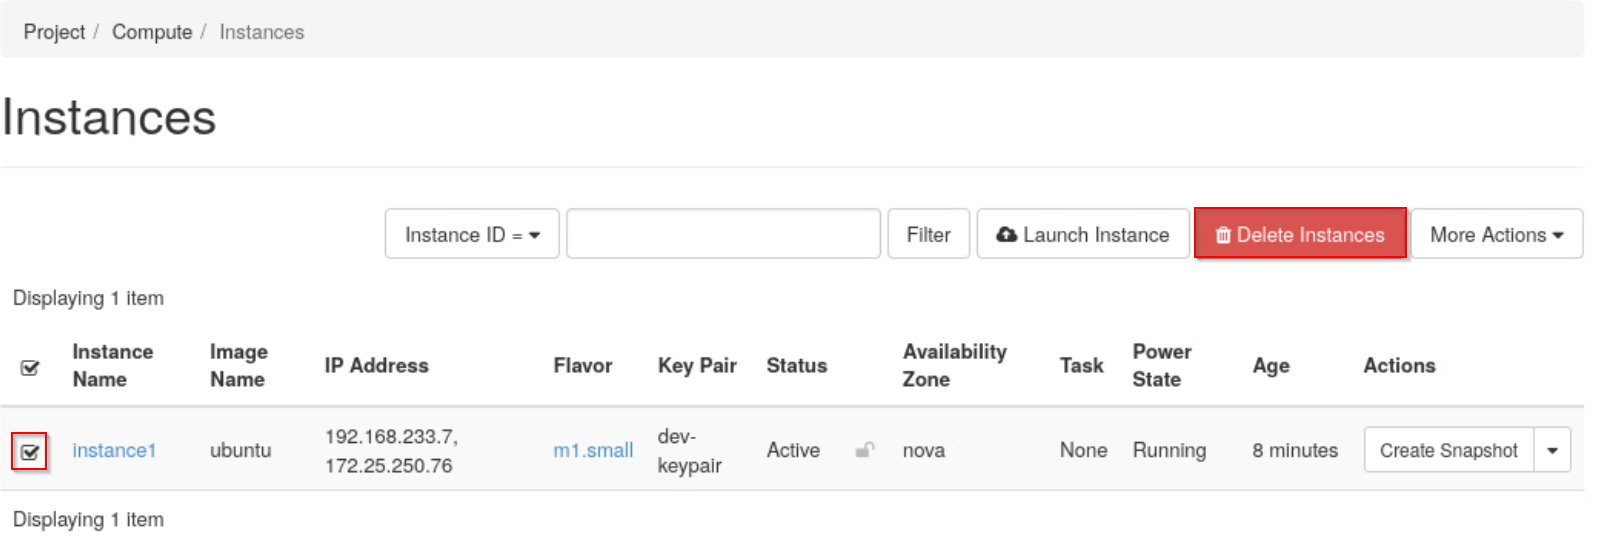
\includegraphics[width=\linewidth]{images/part2/step16.png}
        \end{center}
    \end{labstep}

    \begin{labstep}
        Log out of the \textit{Horizon Dashboard} and close the web browser.
    \end{labstep}

    \begin{labstep}
        Continue to the next task.
    \end{labstep}

\end{enumerate}

%%%%%%%%%%%
% Section 3
%%%%%%%%%%%
\section{Creating a Customized Instance with the OpenStack Unified CLI}\label{sec:creating-a-customized-instance-with-the-openstack-unified-cli}
In this task, you will verify that \textbf{cloud-init} has correctly customized the two instances created in the previous section.

\begin{enumerate}
    \begin{labstep}
        If a terminal window is not already open, open one and source the admin credentials from the \textbf{\texttildemid/keystonerc-admin} file.
        \begin{lstlisting}
            [ubuntu@workstation (keystone-admin)]:~$ source ~/keystonerc-admin
        \end{lstlisting}

        \begin{center}
            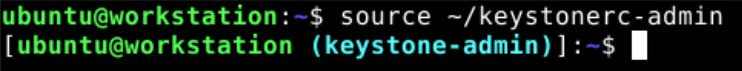
\includegraphics[width=\linewidth]{images/part3/step1.png}
        \end{center}
    \end{labstep}

    \begin{labstep}
        Another instance will be created and customized with the \textit{OpenStack Unified CLI}.
        First, create a \textbf{user-data} script that will be attached to the instance at creation.
        Create a script called \textbf{\texttildemid/hello} that matches the content shown below.
        When the instance runs this script, it will create the file \textbf{/root/hello.txt} with the contents \textbf{Hello, world!}, and it will append the line \textbf{127.0.1.1 instance2} to the \textbf{/etc/hosts} file.
        This simply suppresses a warning when issuing a command with root privileges (i.e., \textbf{sudo …}).
        Press \textbf{CTRL+X}, then \textbf{Y} to accept the file changes.
        Press \textbf{Enter} to confirm and exit back to the terminal.
        \begin{lstlisting}
            [ubuntu@workstation (keystone-admin)]:~$ nano ~/hello
        \end{lstlisting}
        \begin{lstlisting}
            #!/bin/bash
            echo 'Hello, world!' > /root/hello.txt
            echo '127.0.1.1 instance2' >> /etc/hosts
        \end{lstlisting}

        \begin{center}
            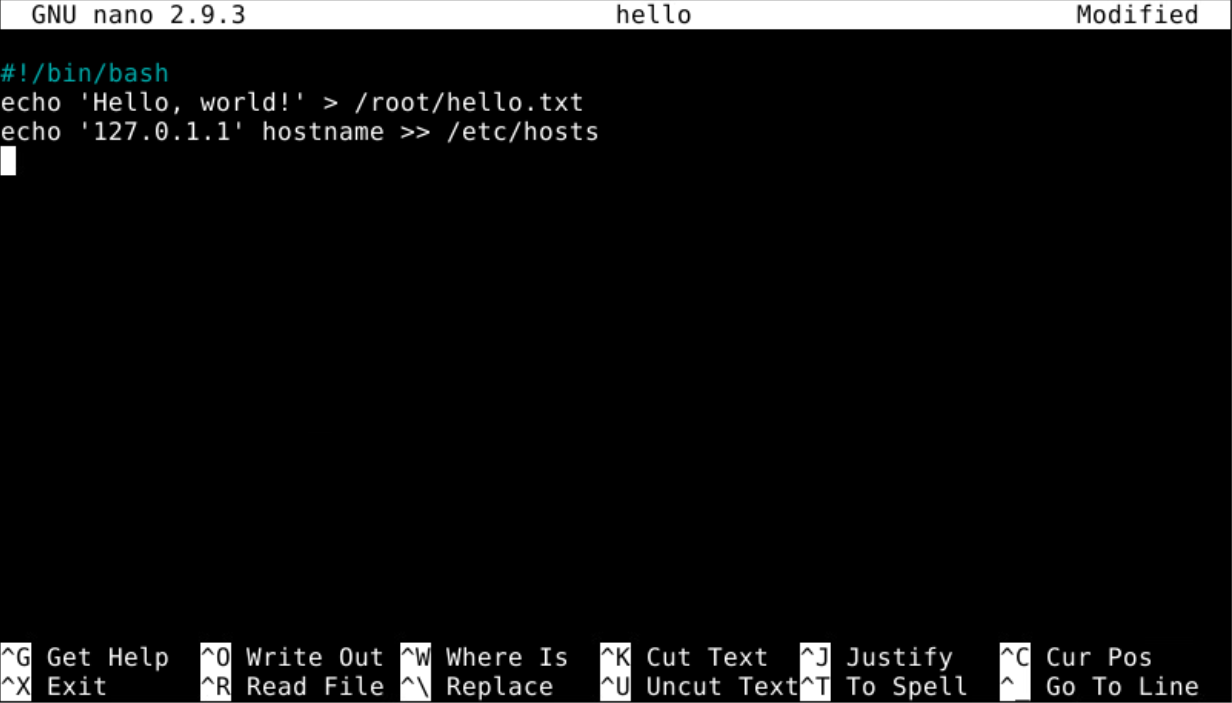
\includegraphics[width=\linewidth]{images/part3/step2.png}
        \end{center}
    \end{labstep}

    \begin{labstep}
        Launch an instance with the \textbf{user-data} option with the previously created script to perform the customization.
        Use the \textbf{ubuntu} image, the \textbf{m1.small} flavor, the \textbf{shared} network, the \textbf{dev-secgroup} security group, and the \textbf{dev-keypair} key pair.
        \begin{lstlisting}
            [ubuntu@workstation (keystone-admin)]:~$ openstack server create \
            > --image ubuntu \
            > --flavor m1.small \
            > --network shared \
            > --security-group dev-secgroup \
            > --key-name dev-keypair \
            > --user-data ~/hello \
            > instance2
        \end{lstlisting}

        \begin{center}
            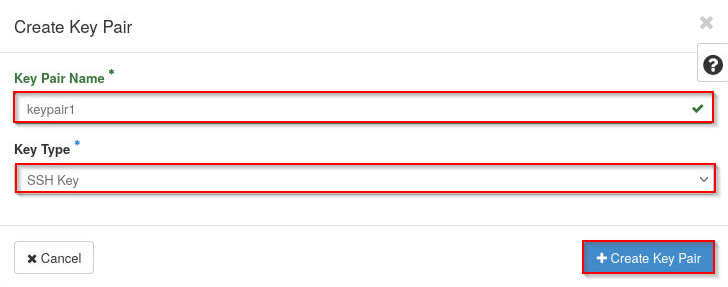
\includegraphics[scale=0.7]{images/part3/step3.png}
        \end{center}
    \end{labstep}

    \begin{labstep}
        Verify that the status of the \textbf{instance2} instance is \textbf{ACTIVE}.
        \begin{lstlisting}
            [ubuntu@workstation (keystone-admin)]:~$ openstack server list
        \end{lstlisting}

        \begin{center}
            \includegraphics[width=\linewidth]{images/part3/step4.png}
        \end{center}
    \end{labstep}

    \begin{labstep}
        List the floating IPs to see the free address, which was disassociated from the previous instance when the instance was deleted.
        \begin{lstlisting}
            [ubuntu@workstation (keystone-admin)]:~$ openstack floating ip list
        \end{lstlisting}

        \begin{center}
            \includegraphics[width=\linewidth]{images/part3/step5.png}
        \end{center}
    \end{labstep}

    \begin{labstep}
        Assign the floating IP to \textbf{instance2}.
        \begin{lstlisting}
            [ubuntu@workstation (keystone-admin)]:~$ openstack server add floating ip \
            > instance2 172.25.250.76
        \end{lstlisting}

        \begin{center}
            \includegraphics[width=\linewidth]{images/part3/step6.png}
        \end{center}
    \end{labstep}

    \begin{labstep}
        Verify that the instance was assigned the floating IP address.
        \begin{lstlisting}
            [ubuntu@workstation (keystone-admin)]:~$ openstack server list \
            > -c Name \
            > -c Networks
        \end{lstlisting}

        \begin{center}
            \includegraphics[width=\linewidth]{images/part3/step7.png}
        \end{center}
    \end{labstep}

    \begin{labstep}
        Use the \textbf{scp} command to copy the \textbf{\texttildemid/Downloads/dev-keypair.pem} file to the \textbf{devstack} machine.
        When prompted to enter the password for \textbf{ubuntu@192.168.1.20}, enter \textbf{ubuntu}.
        \begin{lstlisting}
            [ubuntu@workstation (keystone-admin)]:~$ scp ~/Downloads/dev-keypair.pem \
            > 192.168.1.20:~/dev-keypair.pem
        \end{lstlisting}

        \begin{center}
            \includegraphics[width=\linewidth]{images/part3/step8.png}
        \end{center}
    \end{labstep}

    \begin{labstep}
        SSH into the \textbf{devstack} machine.
        Enter \textbf{ubuntu} when prompted for a password.
        \begin{lstlisting}
            [ubuntu@workstation (keystone-admin)]:~$ ssh 192.168.1.20
        \end{lstlisting}

        \begin{center}
            \includegraphics[width=\linewidth]{images/part3/step9.png}
        \end{center}
    \end{labstep}

    \begin{labstep}
        SSH into \textbf{instance2} with the \textbf{dev-keypair} private key.
        \begin{lstlisting}
            ubuntu@devstack:~$ ssh -i ~/dev-keypair.pem 172.25.250.76
        \end{lstlisting}

        \begin{center}
            \includegraphics[width=\linewidth]{images/part3/step10.png}
        \end{center}
    \end{labstep}

    \begin{notebox}
        It may take several minutes for the instance to fully boot and be available for an SSH connection.
        Until then, the connection will be refused.
    \end{notebox}

    \begin{labstep}
        Check \textbf{/var/log/cloud-init.log} to confirm that the \textbf{cloud-init} script ran.
        \begin{lstlisting}
            ubuntu@instance2:~$ sudo tail /var/log/cloud-init.log
        \end{lstlisting}

        \begin{center}
            \includegraphics[width=\linewidth]{images/part3/step11.png}
        \end{center}
    \end{labstep}

    \begin{labstep}
        View the \textbf{/etc/hosts} file to ensure that the hostname was appended correctly.
        \begin{lstlisting}
            ubuntu@instance2:~$ cat /etc/hosts
        \end{lstlisting}

        \begin{center}
            \includegraphics[width=\linewidth]{images/part3/step12.png}
        \end{center}
    \end{labstep}

    \begin{labstep}
        Ensure that the \textbf{/root/hello.txt} file exists and has the correct content.
        \begin{lstlisting}
            ubuntu@instance2:~$ sudo cat /root/hello.txt
        \end{lstlisting}

        \begin{center}
            \includegraphics[width=\linewidth]{images/part3/step13.png}
        \end{center}
    \end{labstep}

    \begin{labstep}
        The lab is now complete.
    \end{labstep}

\end{enumerate}
\end{document}
